\documentclass[11pt]{article}

\usepackage{latexsym}
\usepackage{amsmath}
\usepackage{amssymb}
\usepackage{amsthm}
\usepackage{graphicx}
\usepackage{wrapfig}
\usepackage{pseudocode}
\usepackage{url}
\usepackage[backref, colorlinks=true, citecolor=red, urlcolor=blue, pdfauthor={Jyh-Ming Lien}]{hyperref}
\usepackage{subfigure}


\newcommand{\handout}[5]{
  \noindent
  \begin{center}
  \framebox{
    \vbox{
      \hbox to 5.78in { {\bf } \hfill #2 }
      \vspace{4mm}
      \hbox to 5.78in { {\Large \hfill #5  \hfill} }
      \vspace{2mm}
      \hbox to 5.78in { {\em #3 \hfill #4} }
    }
  }
  \end{center}
  \vspace*{4mm}
}

\newcommand{\lecture}[4]{\handout{#1}{#2}{#3}{}{Report for #1}}

\newtheorem{theorem}{Theorem}
\newtheorem{corollary}[theorem]{Corollary}
\newtheorem{lemma}[theorem]{Lemma}
\newtheorem{observation}[theorem]{Observation}
\newtheorem{proposition}[theorem]{Proposition}
\newtheorem{definition}[theorem]{Definition}
\newtheorem{claim}[theorem]{Claim}
\newtheorem{fact}[theorem]{Fact}
\newtheorem{assumption}[theorem]{Assumption}

% 1-inch margins, from fullpage.sty by H.Partl, Version 2, Dec. 15, 1988.
\topmargin 0pt
\advance \topmargin by -\headheight
\advance \topmargin by -\headsep
\textheight 8.9in
\oddsidemargin 0pt
\evensidemargin \oddsidemargin
\marginparwidth 0.5in
\textwidth 6.5in

\parindent 0in
\parskip 1.5ex
%\renewcommand{\baselinestretch}{1.25}

\begin{document}

\lecture{Advance Algorithm Programming Assignment 1 }{Fall 2015}{Yeojin Kim}{---}


\section{Implementation Details}
\subsection{algorithm}
The alpha shape algorithm is as follows:
\begin{enumerate}
\item Create points in 4D using 3 coordinates : $\mathbf{(x,y, z, x^2+y^2+z^2)}$
\item Compute convex hull in 4D by calling qhull\cite{Qhull} with 4D points.
\item Looping through all facets in 4D convex hull,
\subitem - Save the vertices of a facets as the vertices of tetrahedron. This vertices are 3 coordinates$\mathbf{(x,y,z)}$.
\subitem - Compute the volume of tetrahedron
\subitem - If the normal vector of tetrahedron points downward and the volume is not zero, compute the radius of circumsphere. Otherwise, continue the loop with new facet.
\subitem - If squared radius is bigger than alpha value, remove tetrahedron. Otherwise, generate faces of tetrahedron. 
\end{enumerate}
\subsection{software}
OS : Window 8.1K\\
IDE : Visual Studio 2013\\
*NOTE :  I use the dynamic library for freeglut.

\section{Example Output}
 Each model was given three different alpha values. In Fig. \ref{fig:cube} - Fig. \ref{fig:teeth}, the alpha value increases through (a) - (c). The exact alpha values are shown in Table \ref{table:alphavalues}.
 \begin{table}[htb]
 \caption{Alpha values of each model.}
 \begin{center}
 \begin{tabular}{|c|c|c|c|}
 \hline
 Model & (a)Alpha1 & (b)Alpha2 & (3)Alpha3 \\
 \hline
 cube & 50 & 78 & - \\
 \hline
 ellipsoid & 5000 & 10000 & 1E+5 \\
 \hline
 bunny & 1000 & 10000 & 1E+6 \\
 \hline
 U & 100 & 10000 & 1E+6 \\
 \hline
 bull & 1E+5 & 1E+6 & 1E+7 \\
 \hline
 baby & 100 & 10000 & 1E+6 \\
 \hline
 woman & 100 & 10000 & 1E+6 \\
 \hline
 T & 10000 & 15000 & 1E+5 \\
 \hline
 Y & 1000 & 10000 & 1E+5 \\
 \hline
 screwdriver & 10000 & 1E+6 & 1E+8 \\
 \hline
 spoon & 10000 & 1E+9 & 1E+13 \\
 \hline
 teeth & 1000 & 1E+6 & 1E+9 \\
 \hline
 \end{tabular}
 \end{center}
 \label{table:alphavalues}
 \end{table} 
\section{Know bugs/limitations}
 In case of cube (Fig. \ref{fig:cube}), it is a degenerate case that all the tetrahedra is on the same circumsphere. Therefore, it removes all the faces after specific radius. 
 
\bibliographystyle{plain}
\bibliography{report}

\begin{figure*}[hbt]
 \centering
  \subfigure[]{
    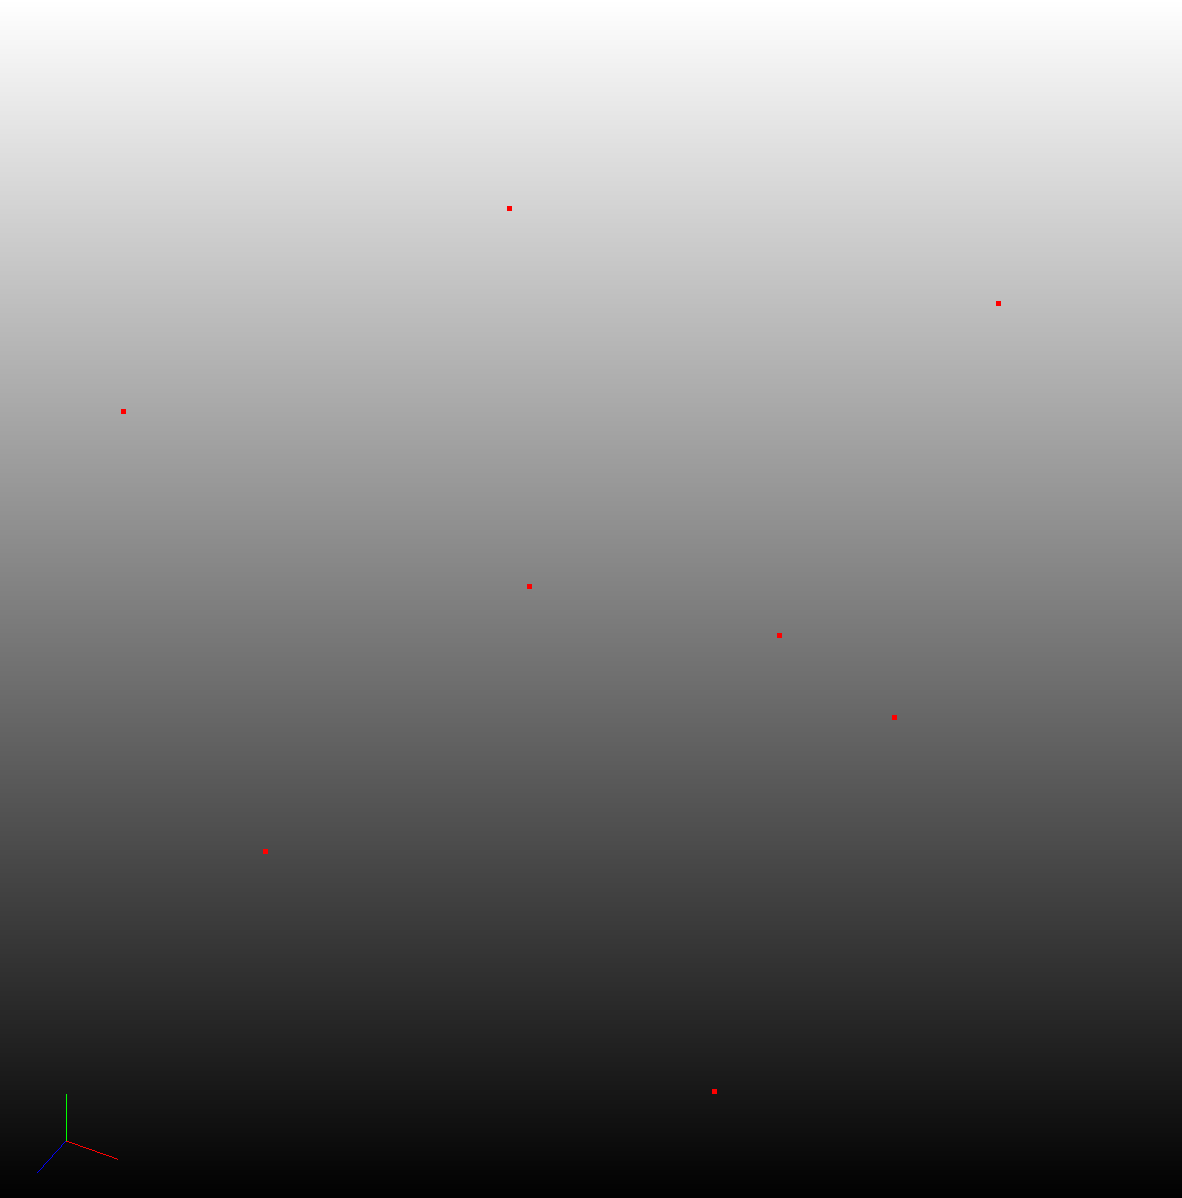
\includegraphics[width=0.42\textwidth]{img/cube1.png}
    \label{fig:cube1}
  }\hspace{-3mm}
  \subfigure[]{
     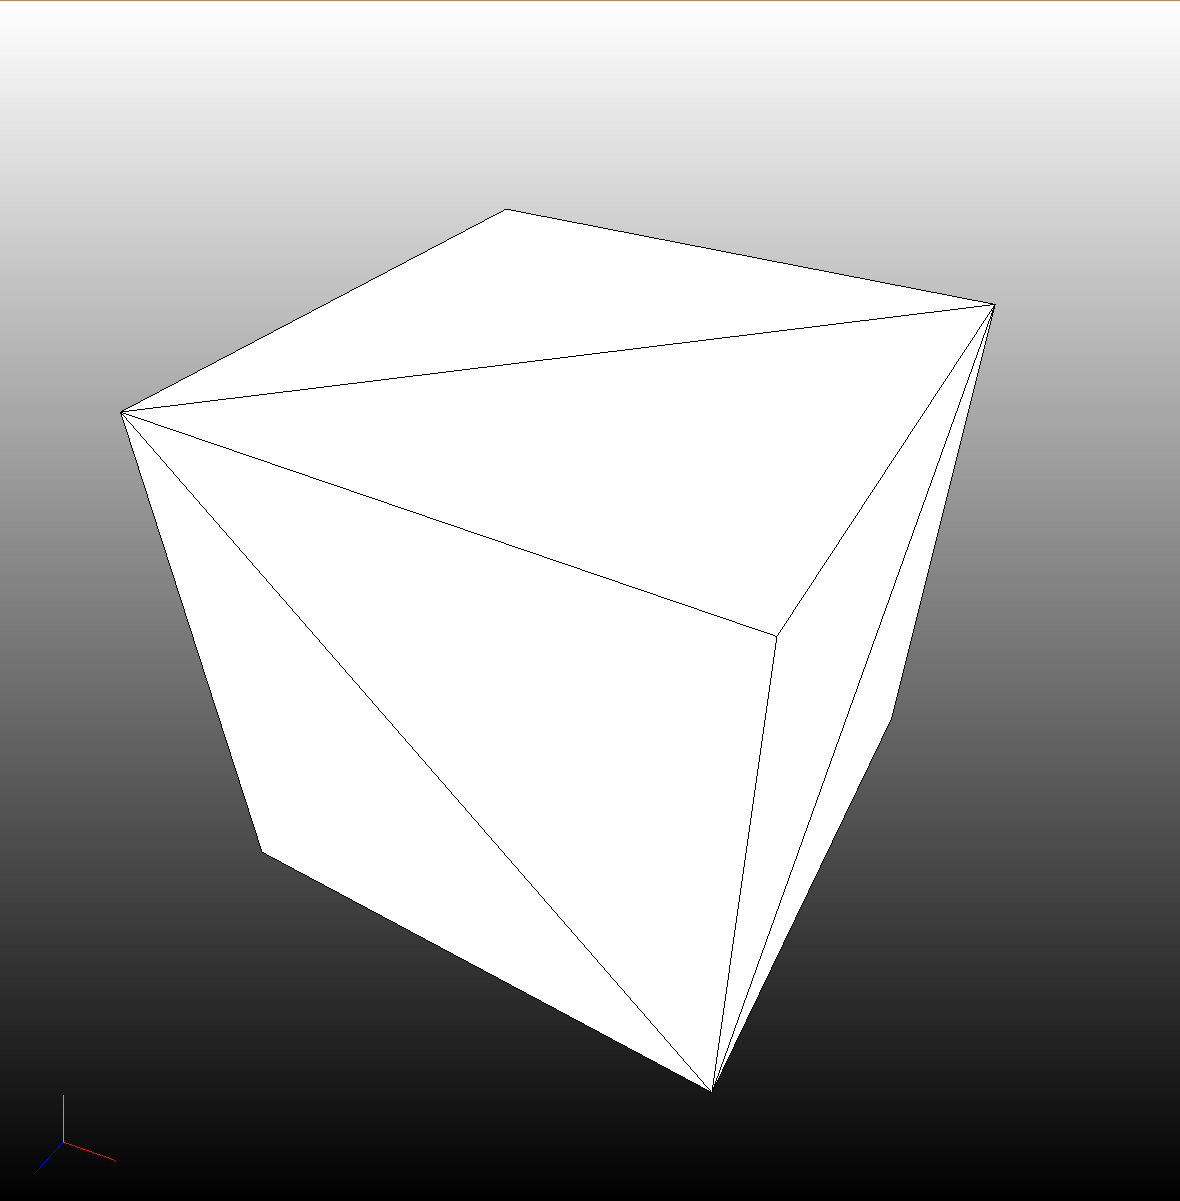
\includegraphics[width=0.42\textwidth]{img/cube2.png}
     \label{fig:cube2}
  }\hspace{-3mm}
    \caption{A cube example\label{fig:cube}}
\end{figure*}
\begin{figure*}[hbt]
 \centering
  \subfigure[]{
    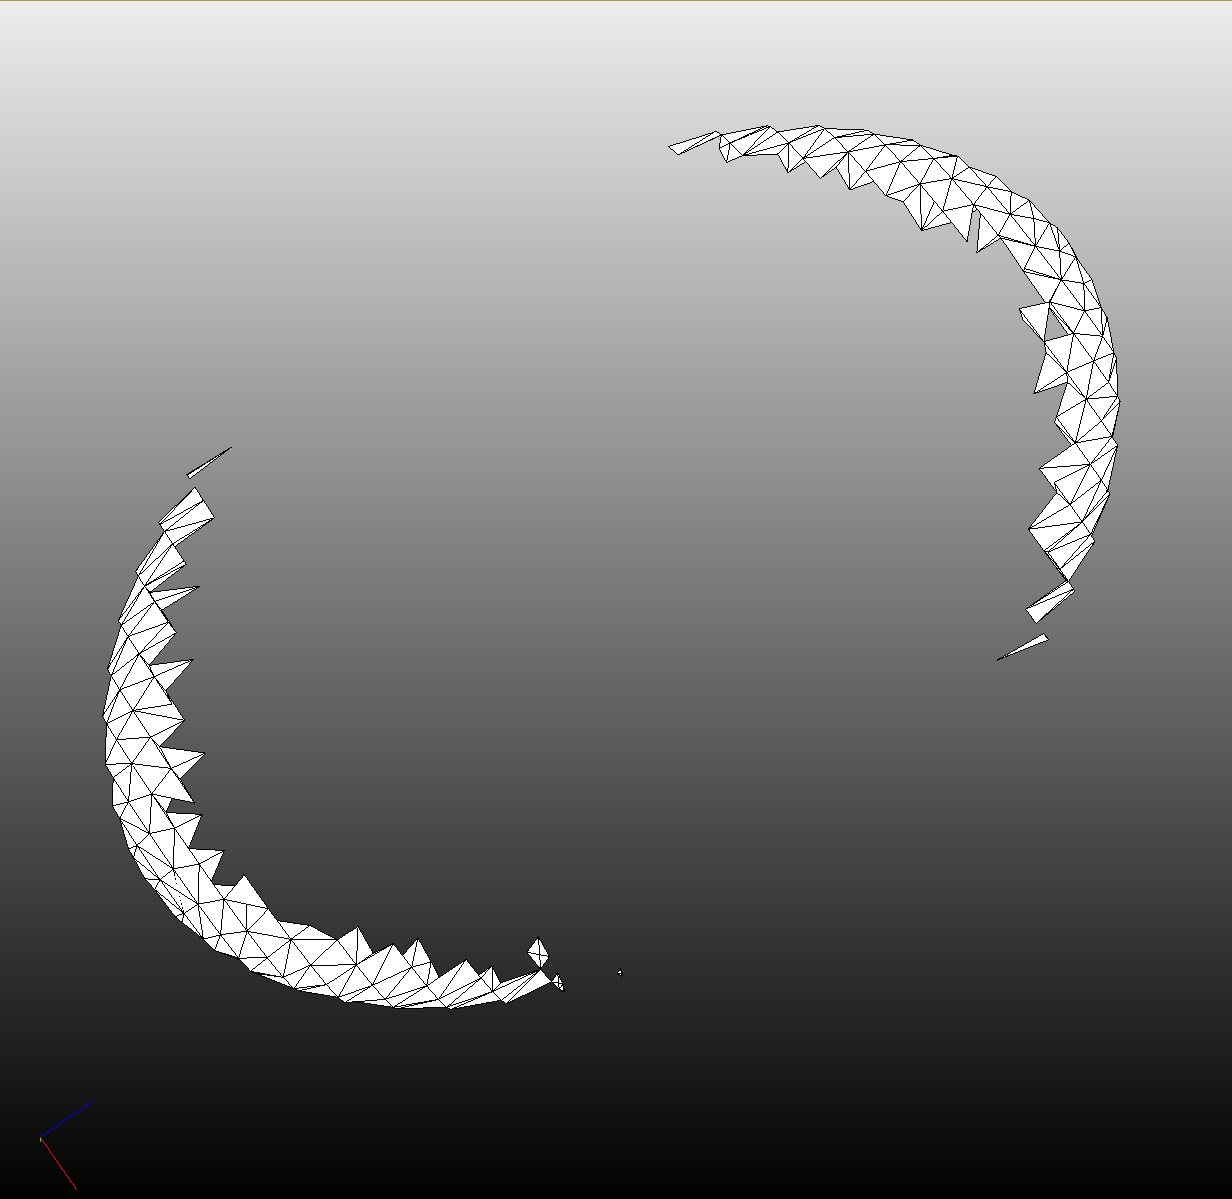
\includegraphics[width=0.32\textwidth]{img/ellipsoid1.png}
    \label{fig:ellipsoid1}
  }\hspace{-3mm}
  \subfigure[]{
     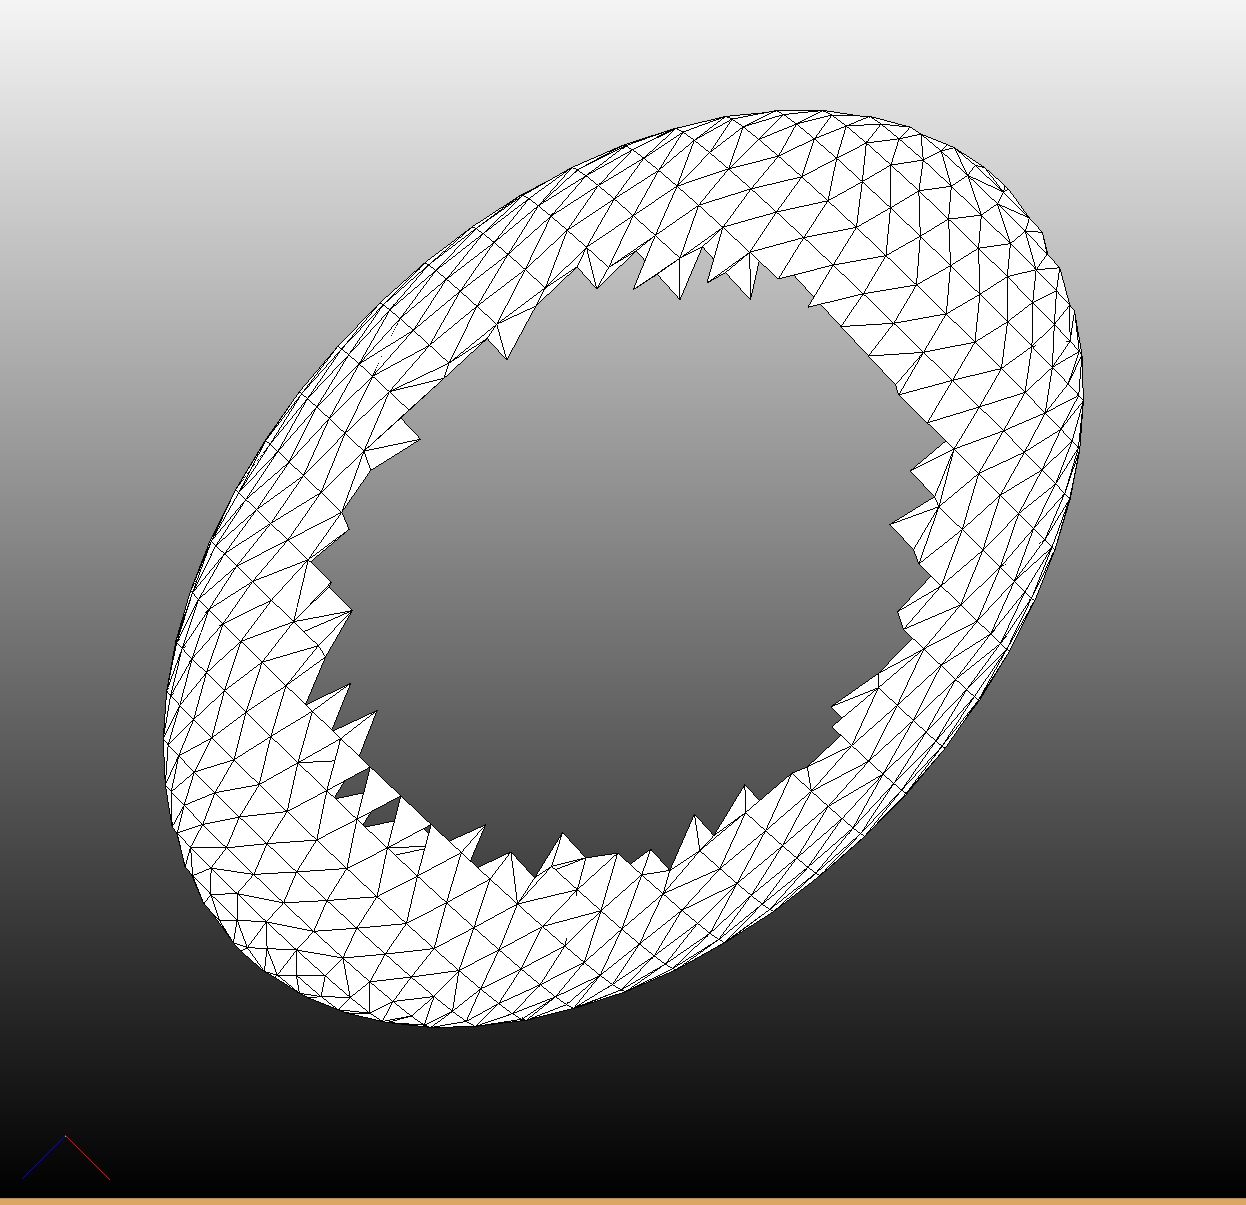
\includegraphics[width=0.32\textwidth]{img/ellipsoid2.png}
     \label{fig:ellipsoid2}
  }\hspace{-3mm}
  \subfigure[]{
    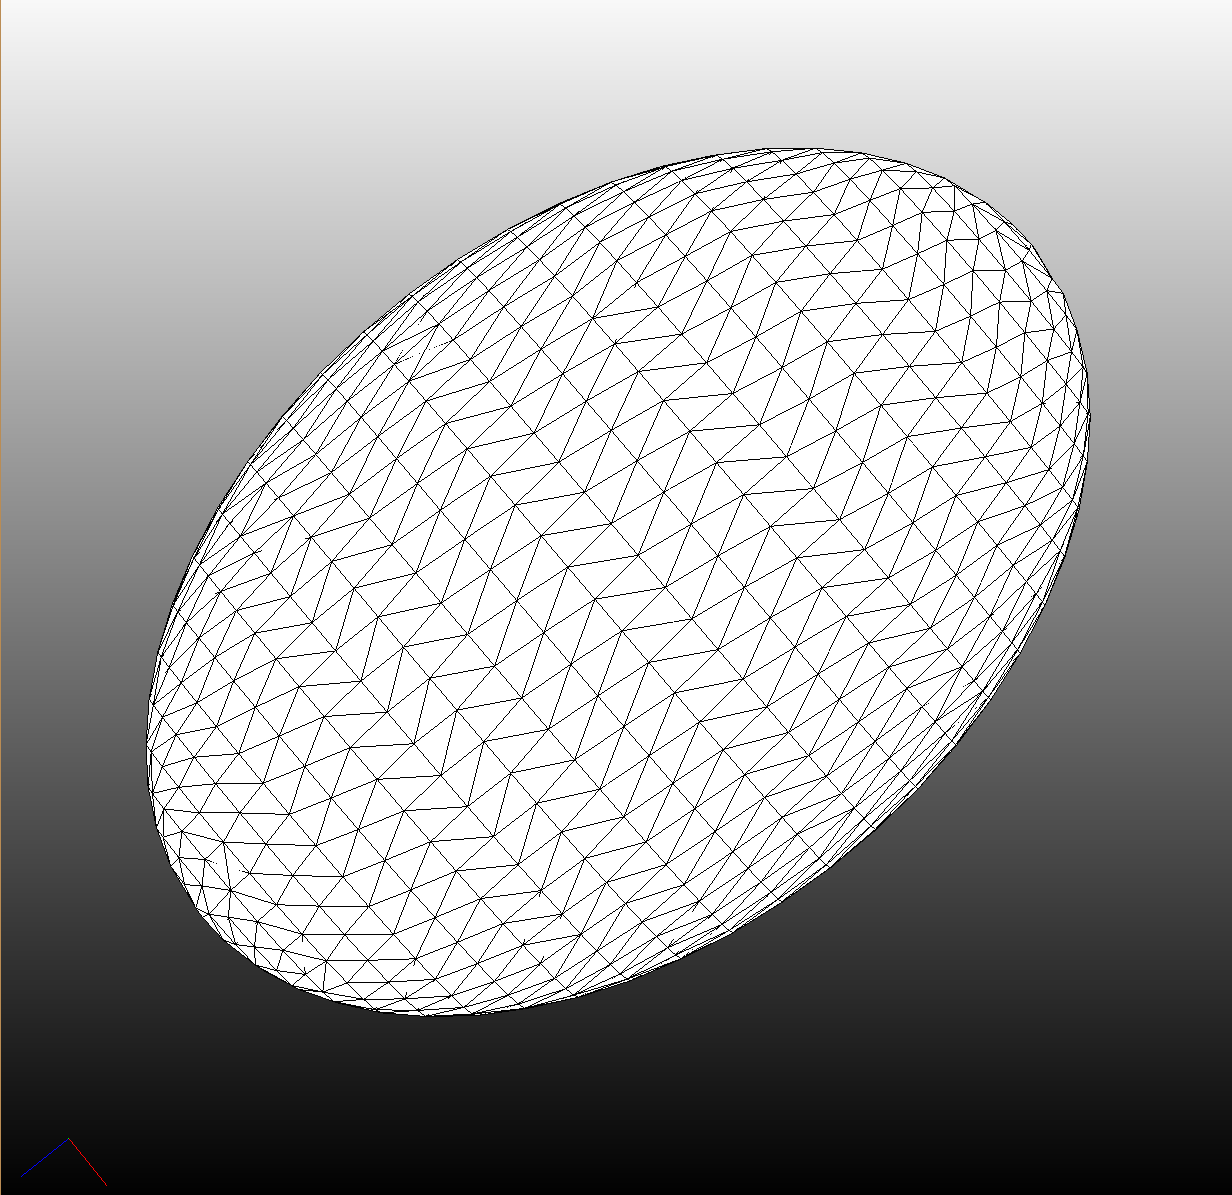
\includegraphics[width=0.32\textwidth]{img/ellipsoid3.png}
     \label{fig:ellipsoid3}
  }\hspace{-3mm}
  \caption{An ellipsoid example \label{fig:ellipsoid}}
\end{figure*}
\begin{figure*}[hbt]
 \centering
  \subfigure[]{
    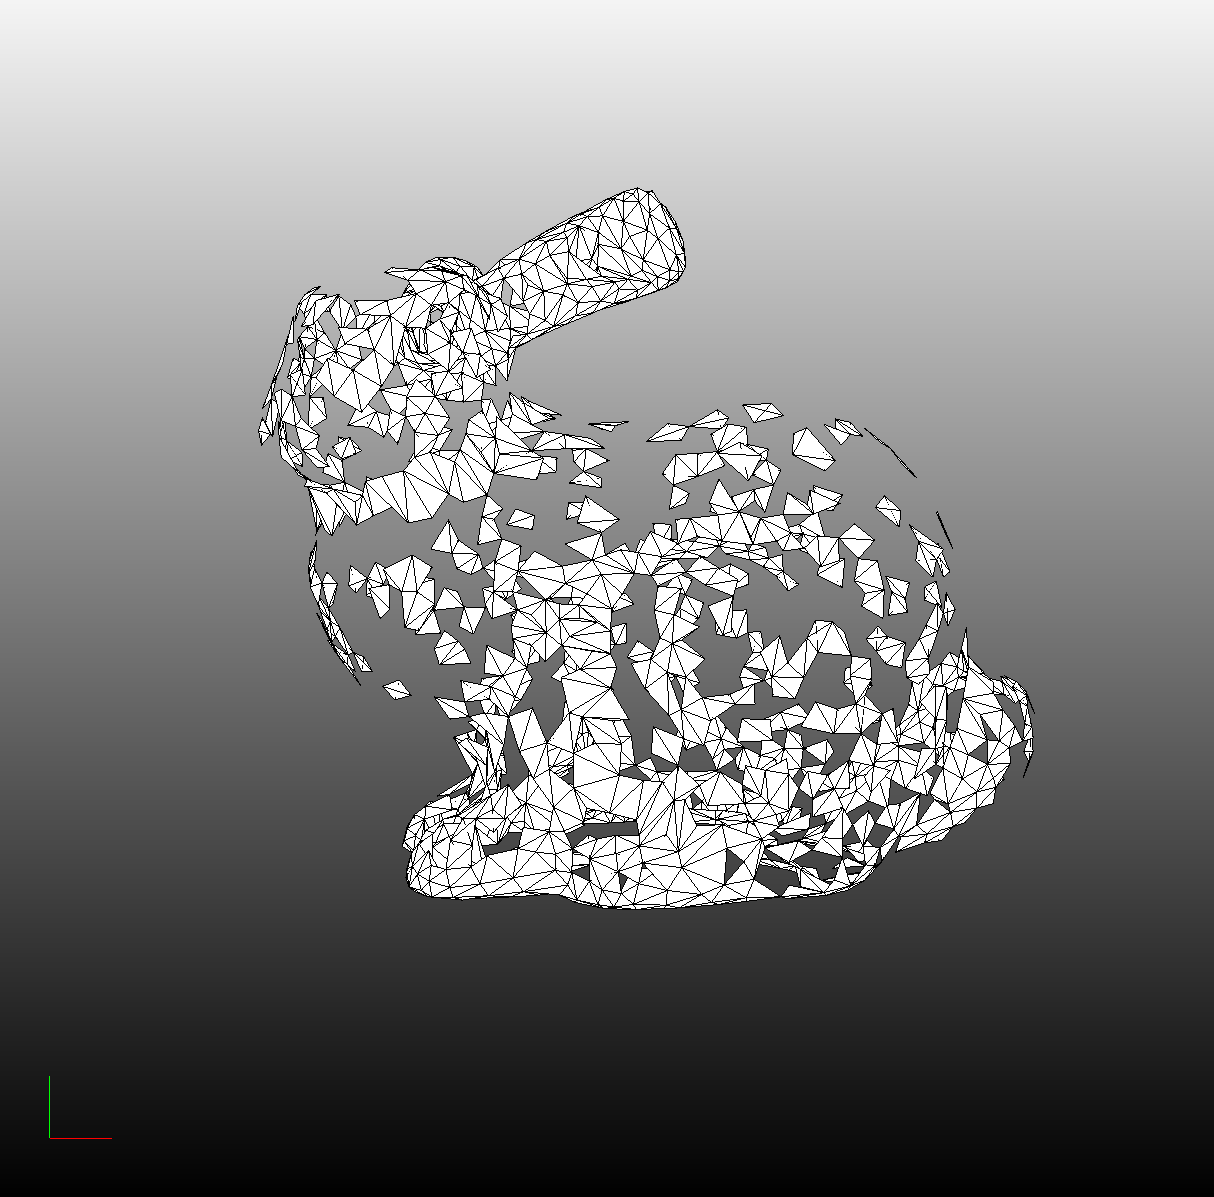
\includegraphics[width=0.32\textwidth]{img/bunny1.png}
    \label{fig:bunny1}
  }\hspace{-3mm}
  \subfigure[]{
     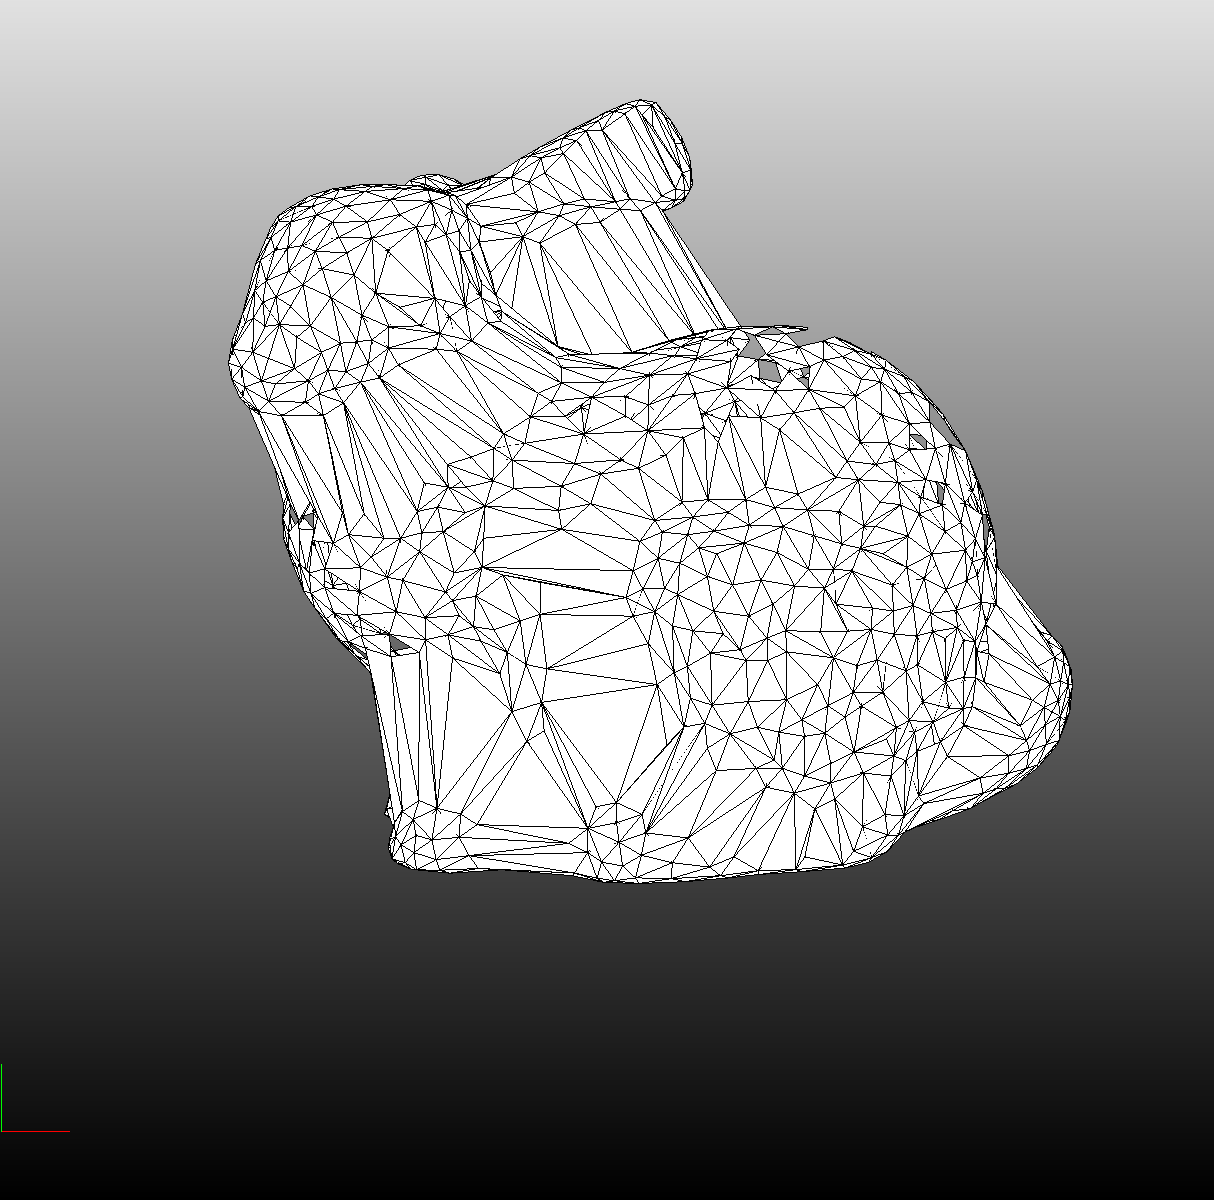
\includegraphics[width=0.32\textwidth]{img/bunny2.png}
     \label{fig:bunny2}
  }\hspace{-3mm}
  \subfigure[]{
    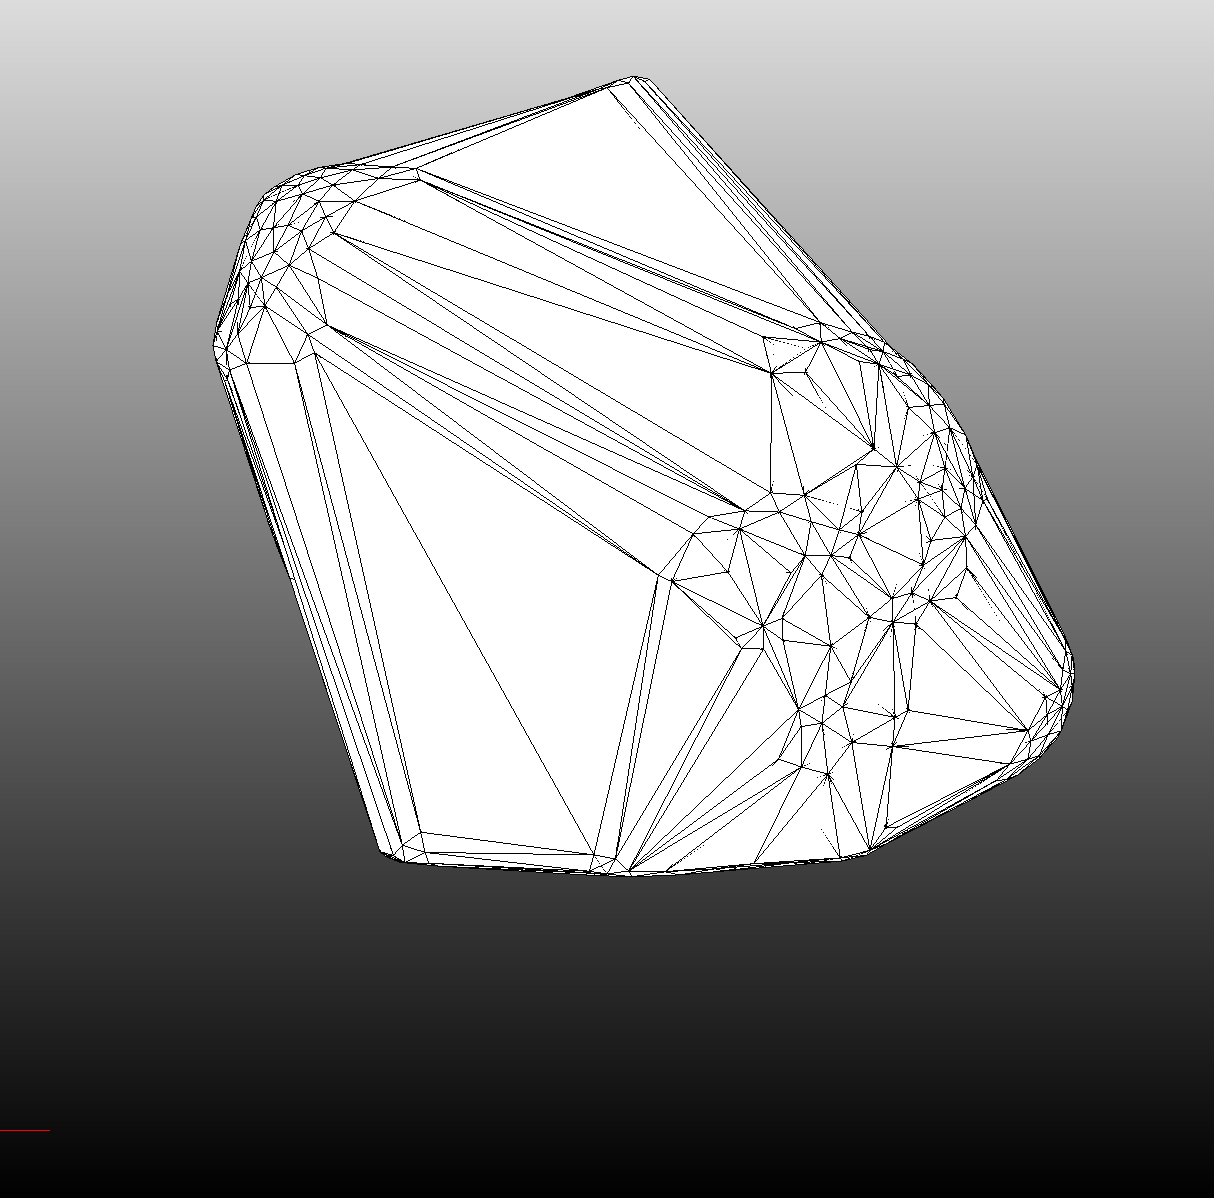
\includegraphics[width=0.32\textwidth]{img/bunny3.png}
     \label{fig:bunny3}
  }\hspace{-3mm}
  \caption{A bunny example \label{fig:bunny}}
\end{figure*}
\begin{figure*}[hbt]
 \centering
  \subfigure[]{
    
\includegraphics[width=0.32\textwidth]{img/U1.png}
    \label{fig:u1}
  }\hspace{-3mm}
  \subfigure[]{
     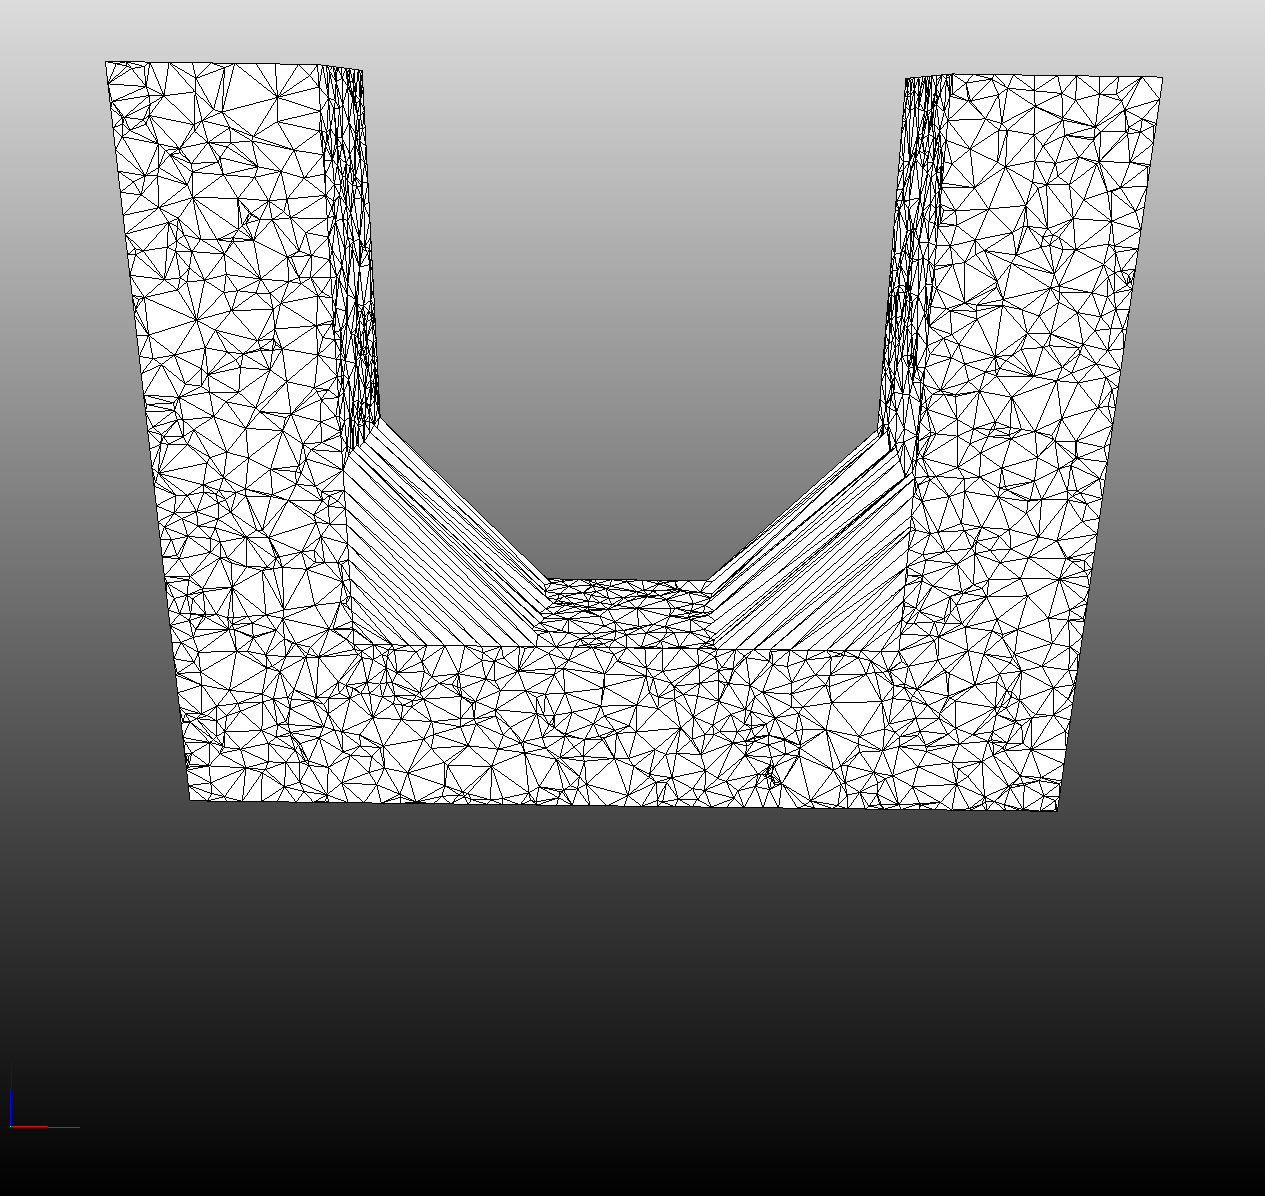
\includegraphics[width=0.32\textwidth]{img/U2.png}
     \label{fig:u2}
  }\hspace{-3mm}
  \subfigure[]{
    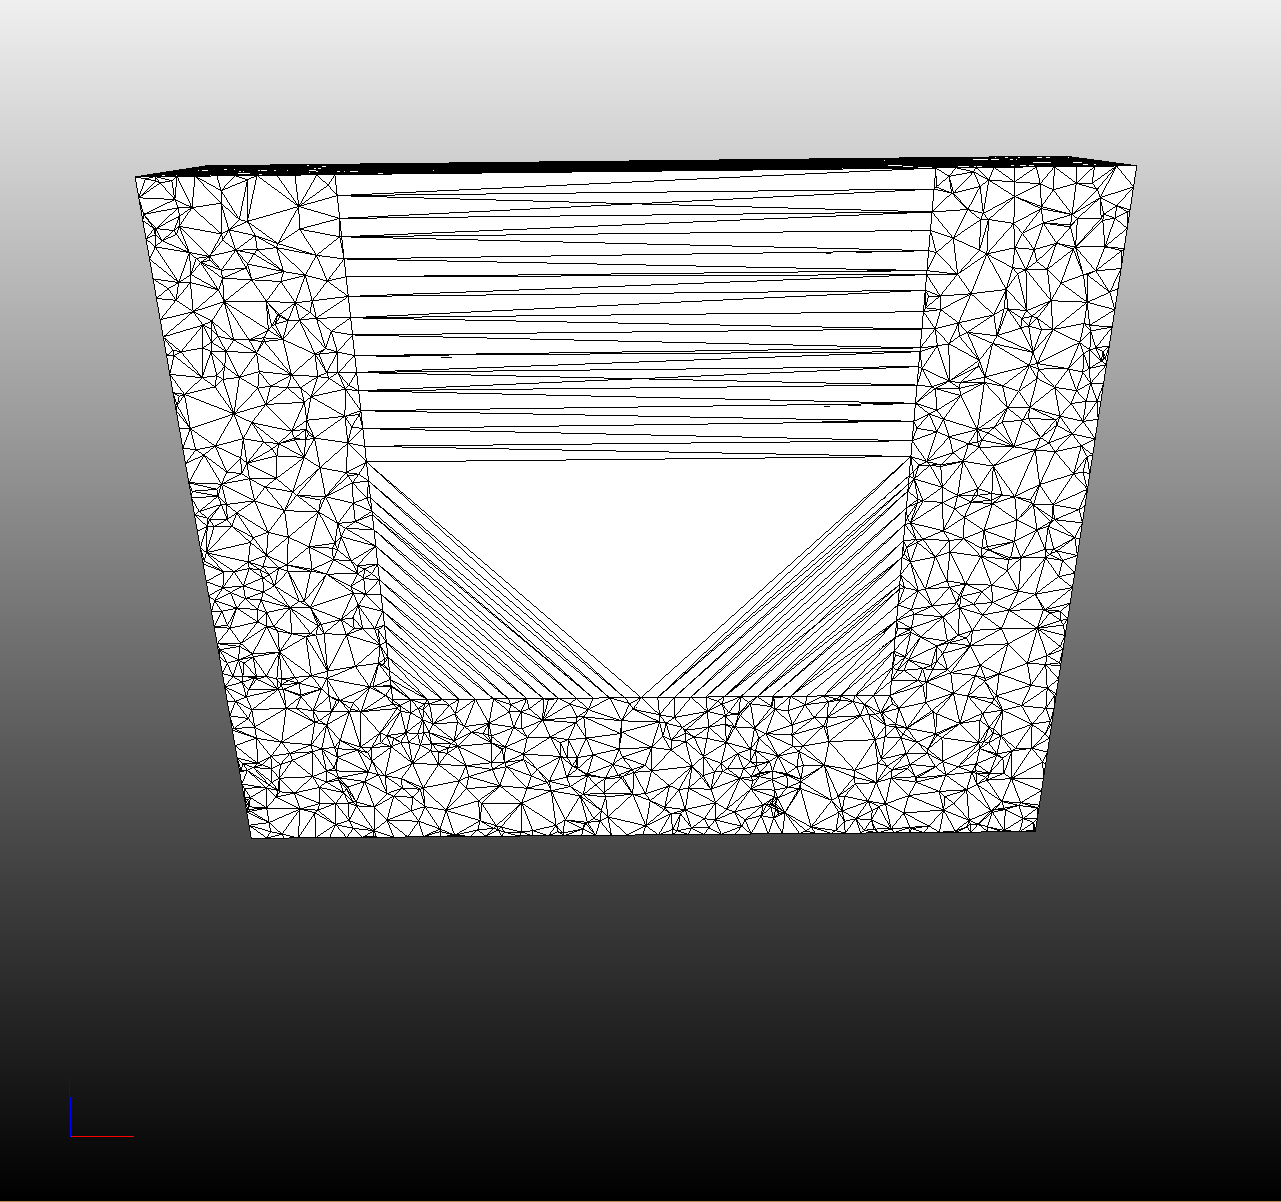
\includegraphics[width=0.32\textwidth]{img/U3.png}
     \label{fig:u3}
  }\hspace{-3mm}
  \caption{An 'U' example \label{fig:U}}
\end{figure*}
\begin{figure*}[hbt]
 \centering
  \subfigure[]{
    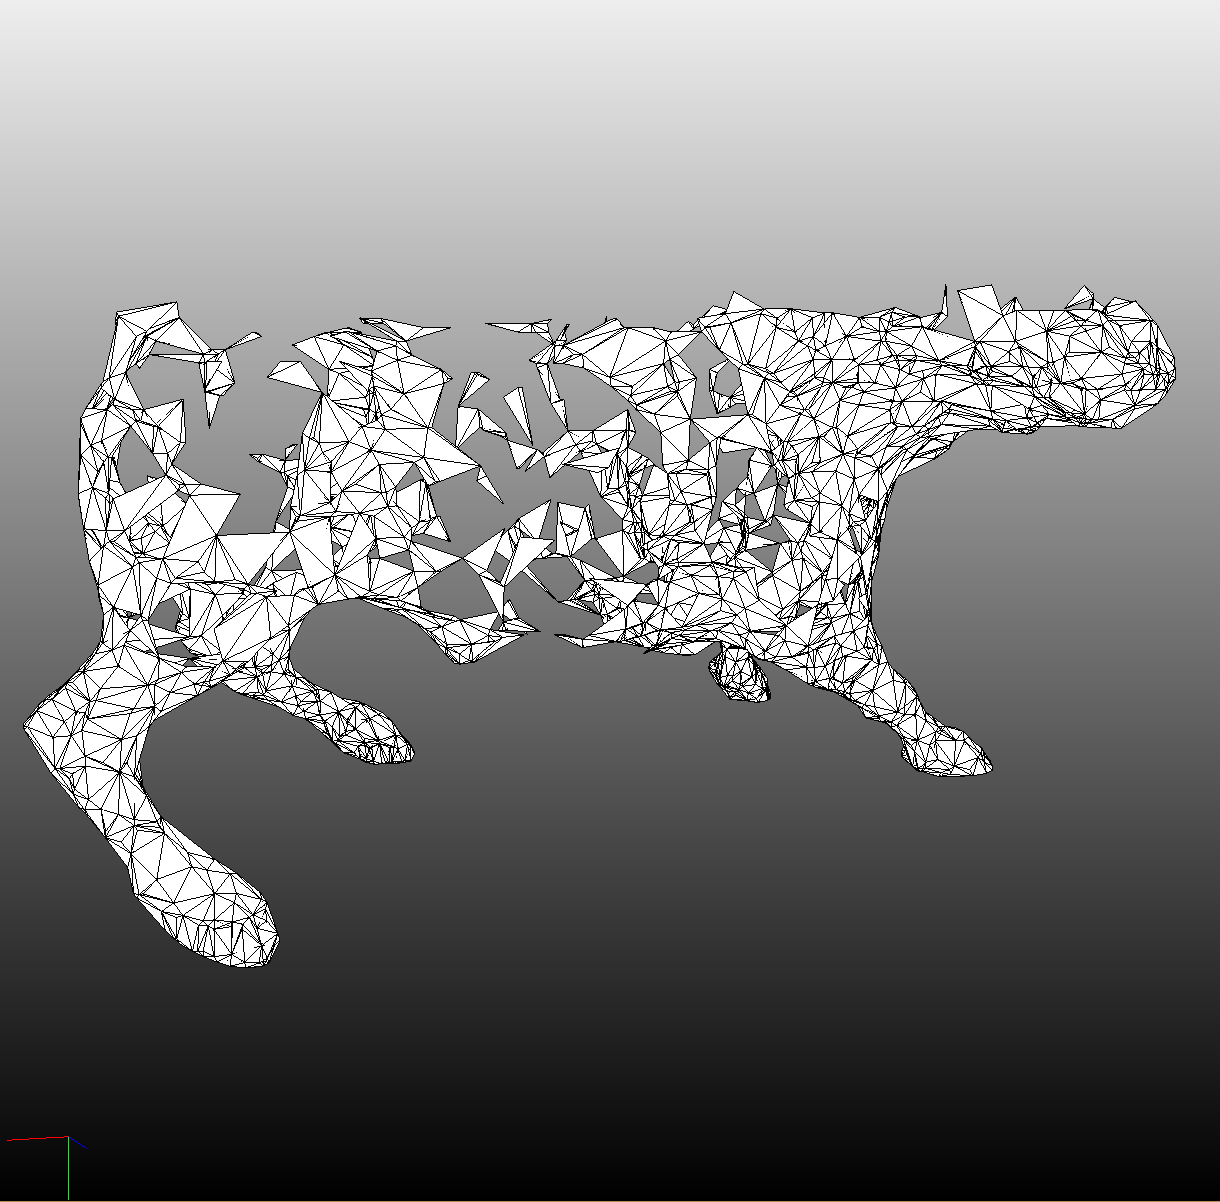
\includegraphics[width=0.32\textwidth]{img/bull1.png}
    \label{fig:bull1}
  }\hspace{-3mm}
  \subfigure[]{
     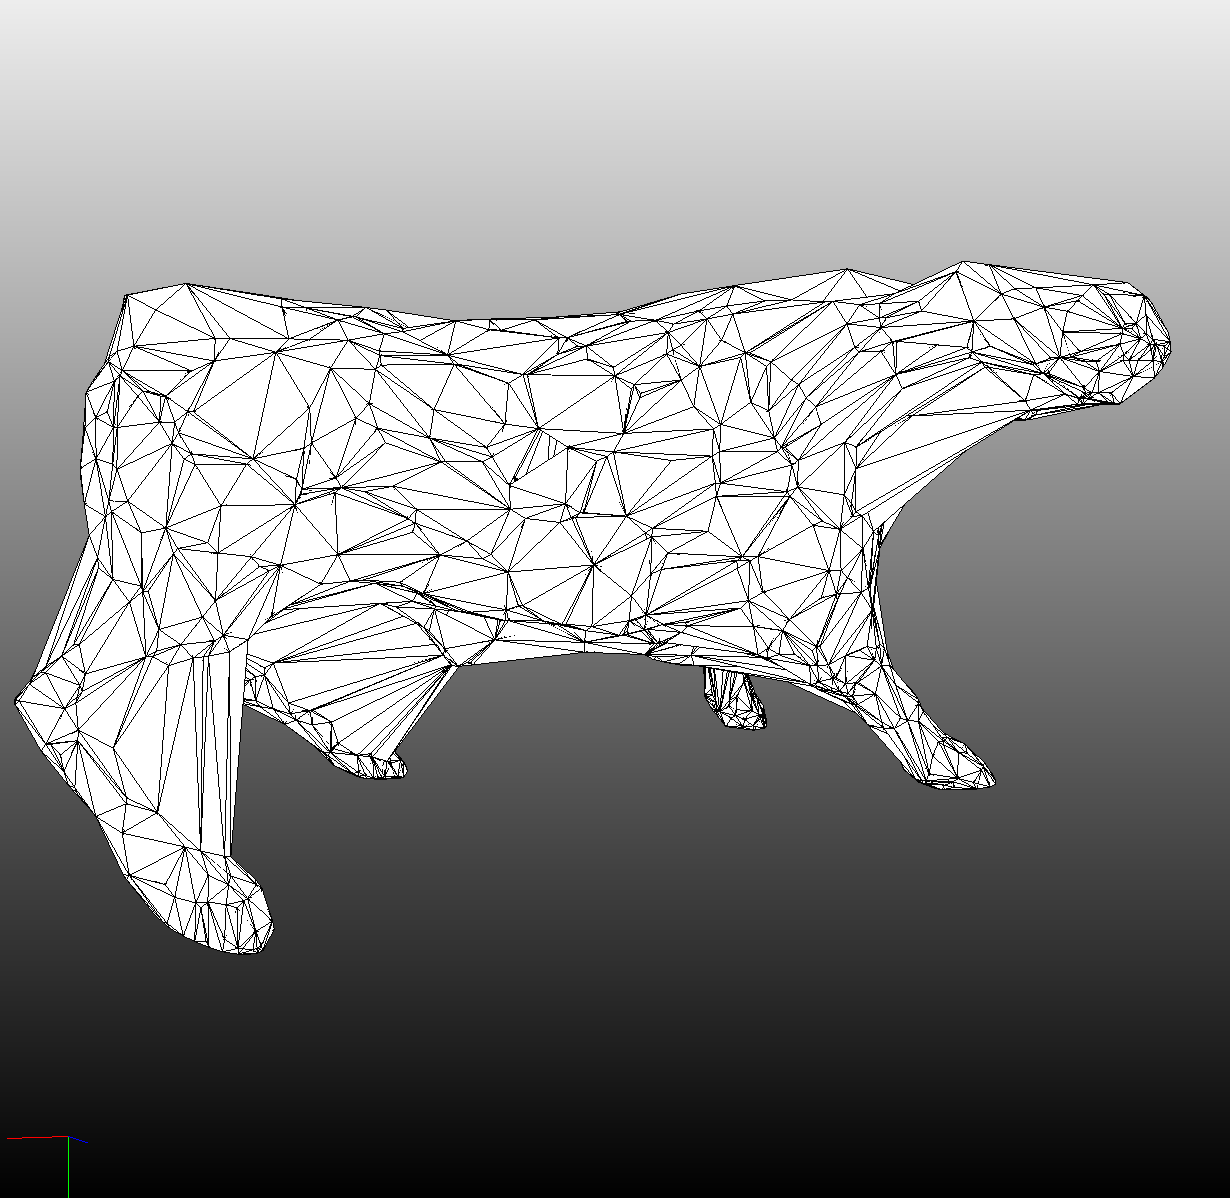
\includegraphics[width=0.32\textwidth]{img/bull2.png}
     \label{fig:bull2}
  }\hspace{-3mm}
  \subfigure[]{
    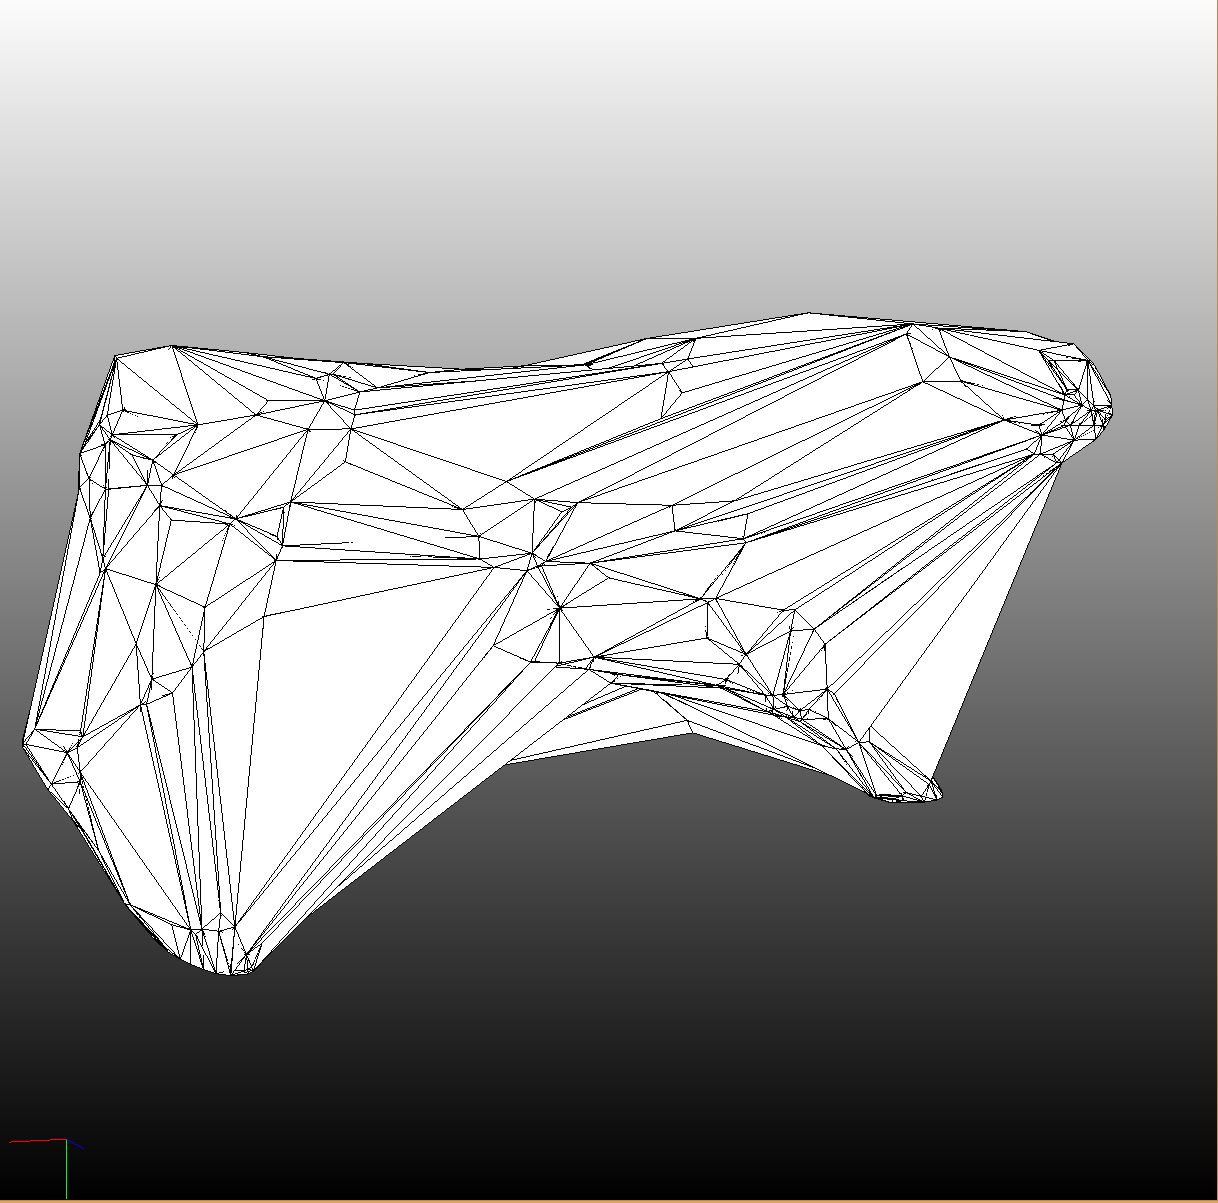
\includegraphics[width=0.32\textwidth]{img/bull3.png}
     \label{fig:bull3}
  }\hspace{-3mm}
  \caption{A bull example \label{fig:bull}}
\end{figure*}
\begin{figure*}[hbt]
 \centering
  \subfigure[]{
    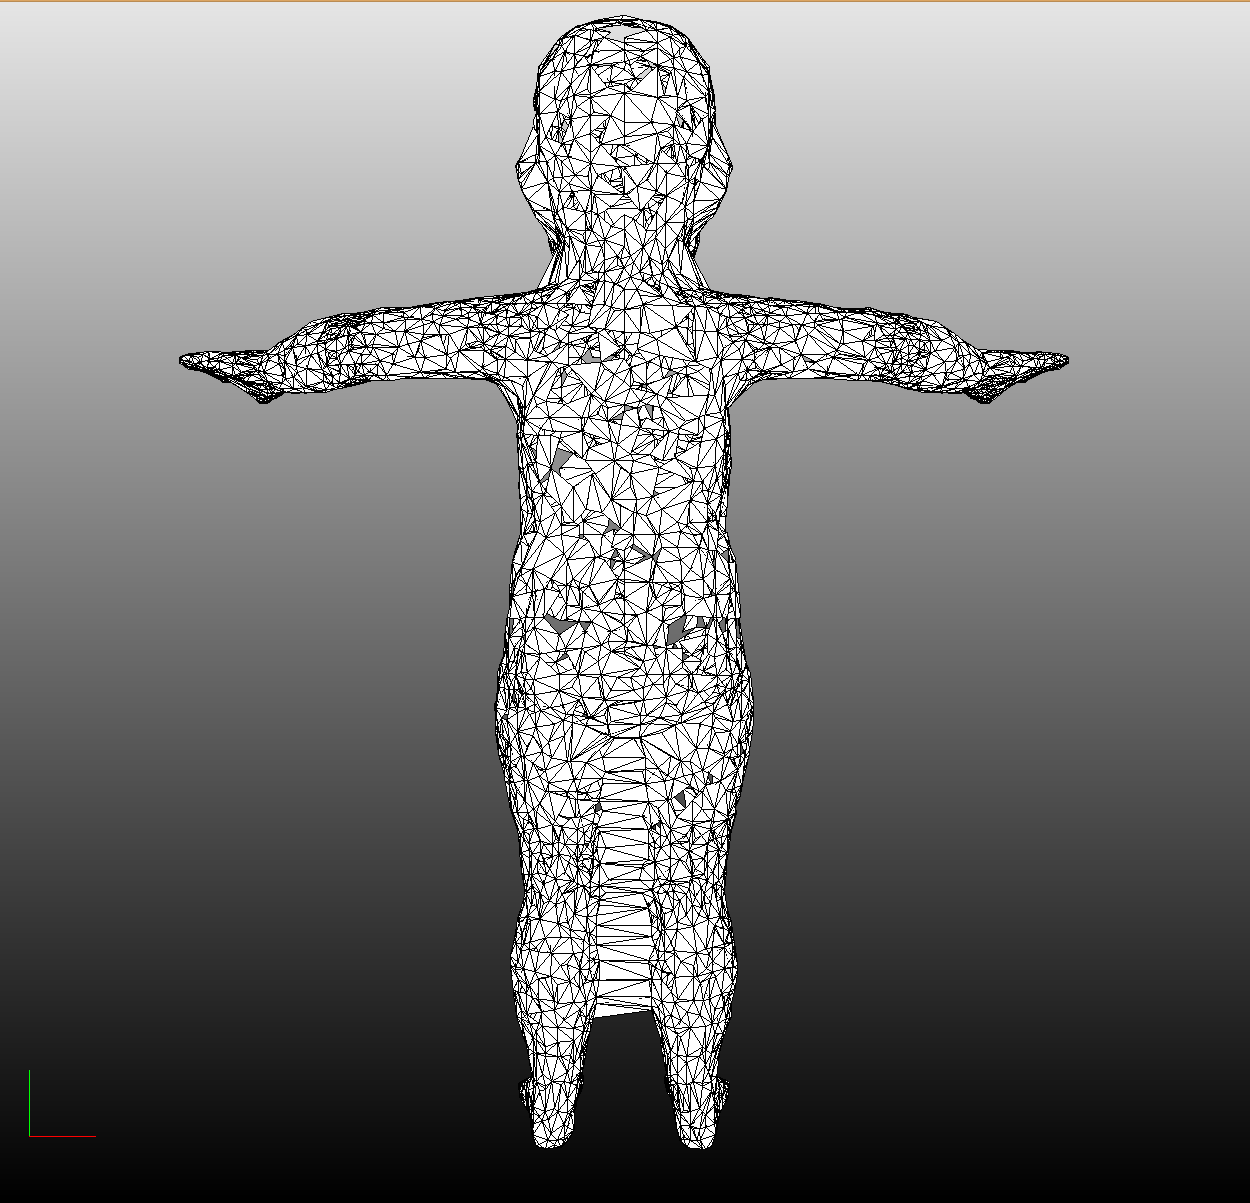
\includegraphics[width=0.32\textwidth]{img/bb1.png}
    \label{fig:bb1}
  }\hspace{-3mm}
  \subfigure[]{
     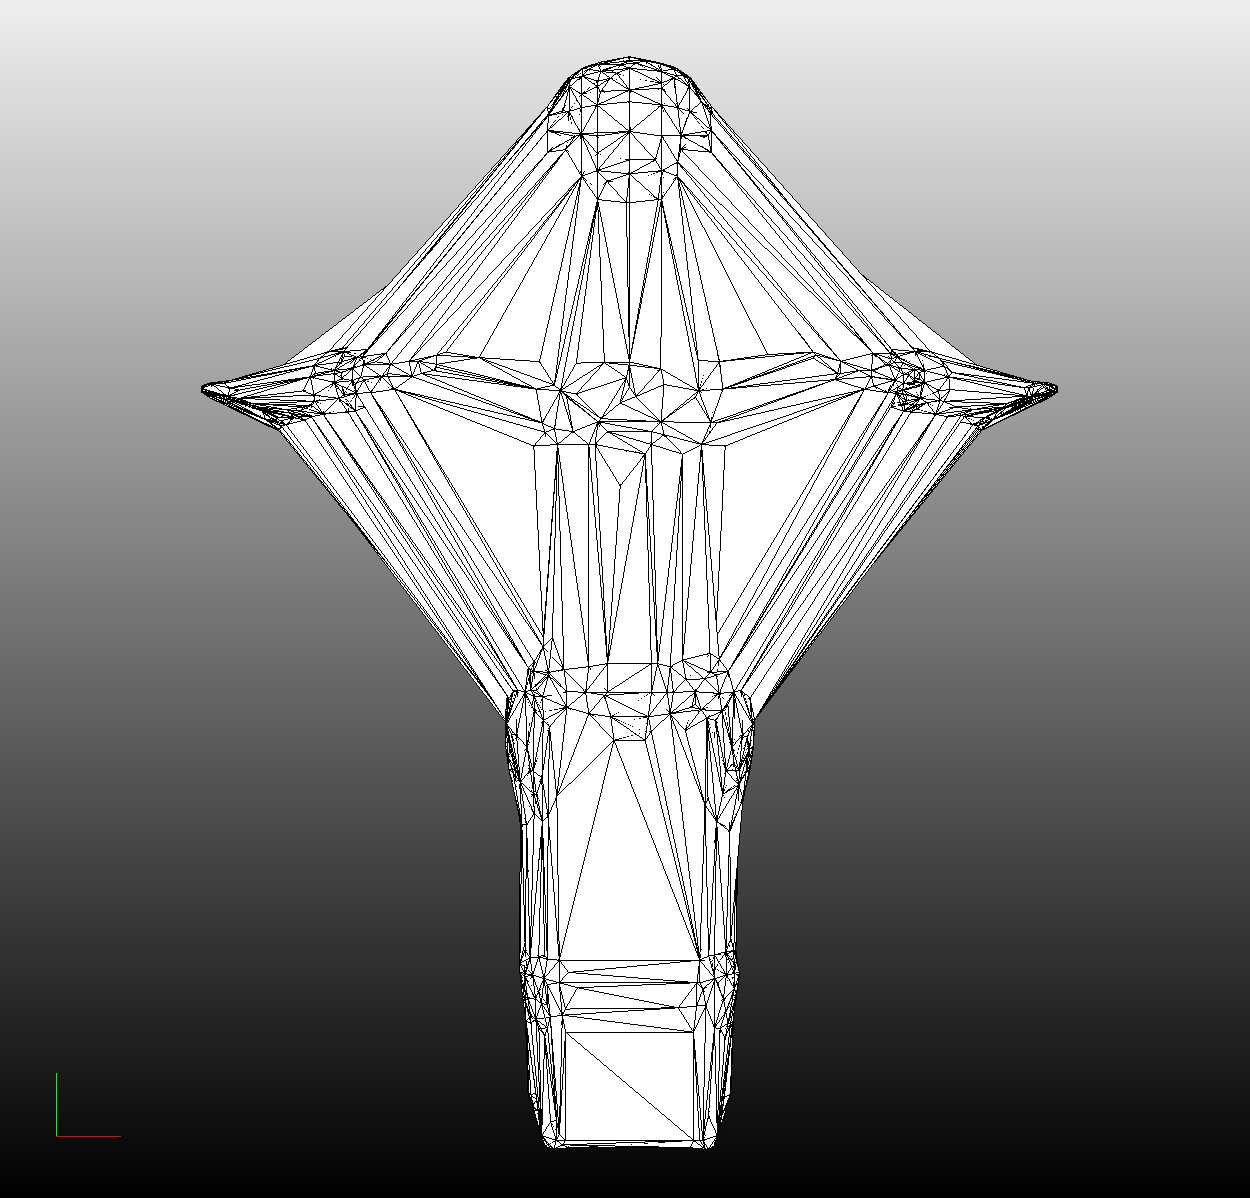
\includegraphics[width=0.32\textwidth]{img/bb2.png}
     \label{fig:bb2}
  }\hspace{-3mm}
  \subfigure[]{
    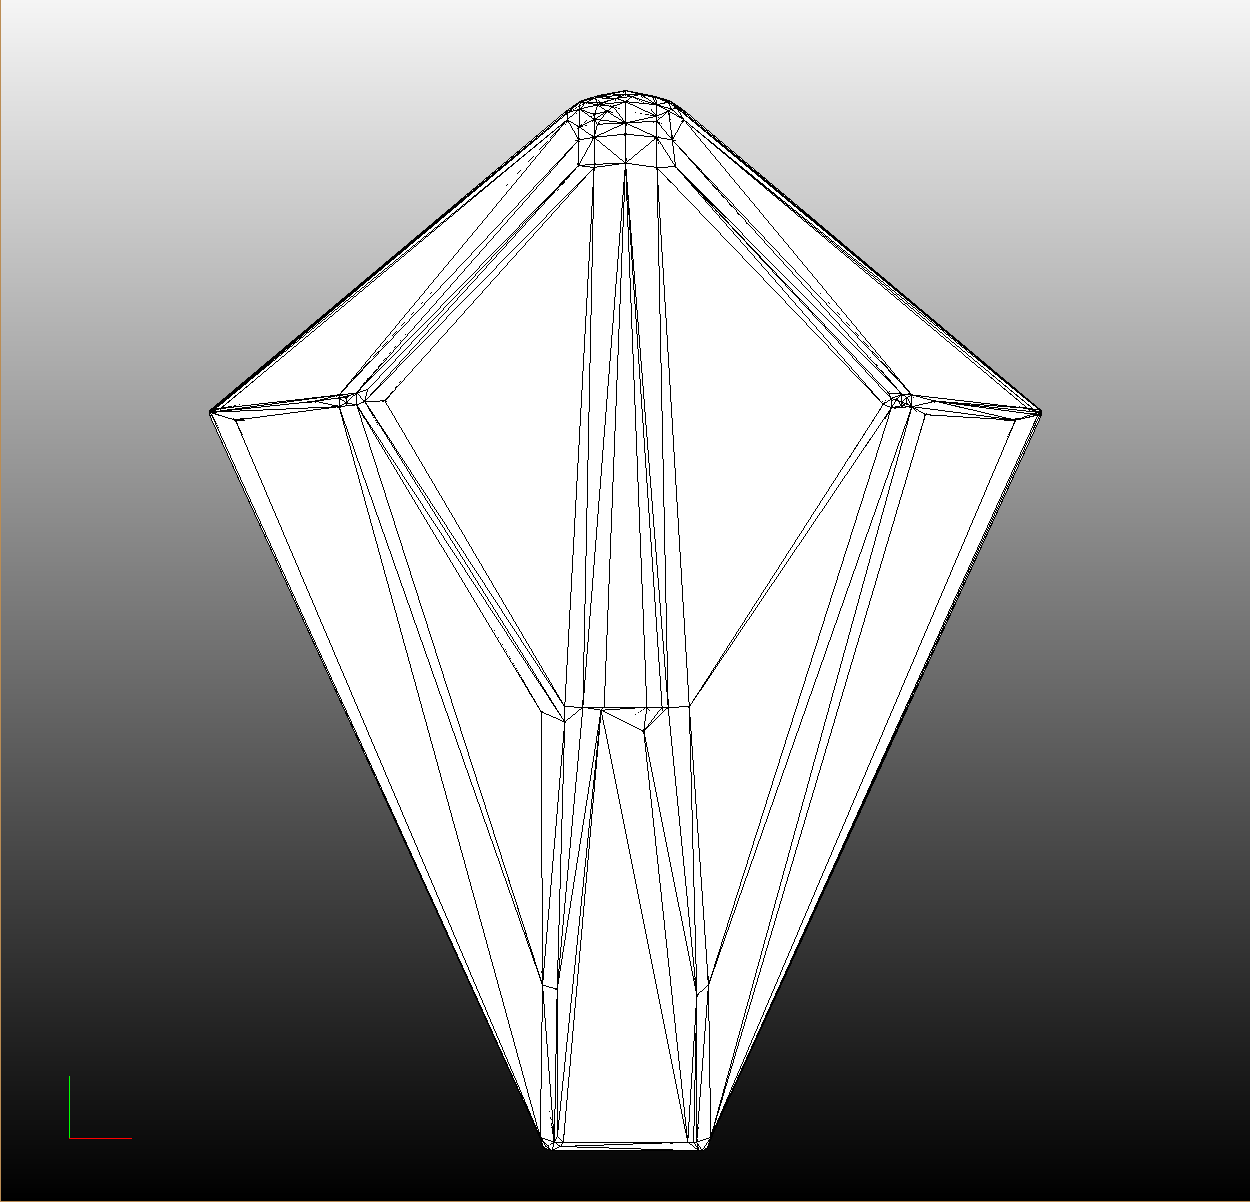
\includegraphics[width=0.32\textwidth]{img/bb3.png}
     \label{fig:bb3}
  }\hspace{-3mm}
  \caption{An baby example \label{fig:baby}}
\end{figure*}
\begin{figure*}[hbt]
 \centering
  \subfigure[]{
    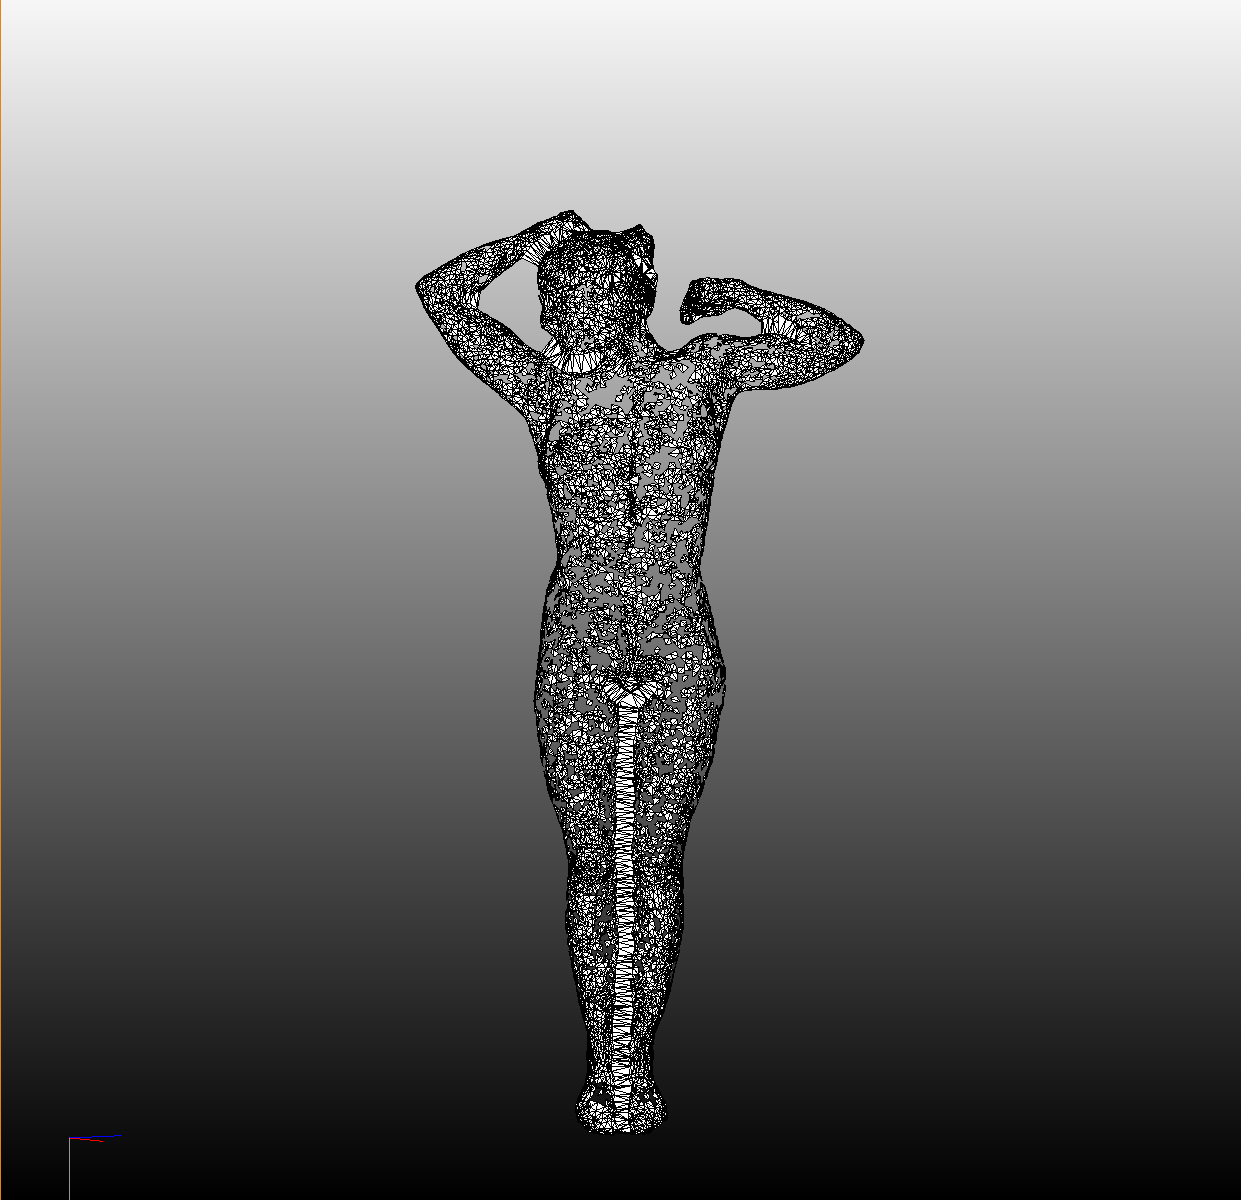
\includegraphics[width=0.32\textwidth]{img/woman1.png}
    \label{fig:woman1}
  }\hspace{-3mm}
  \subfigure[]{
     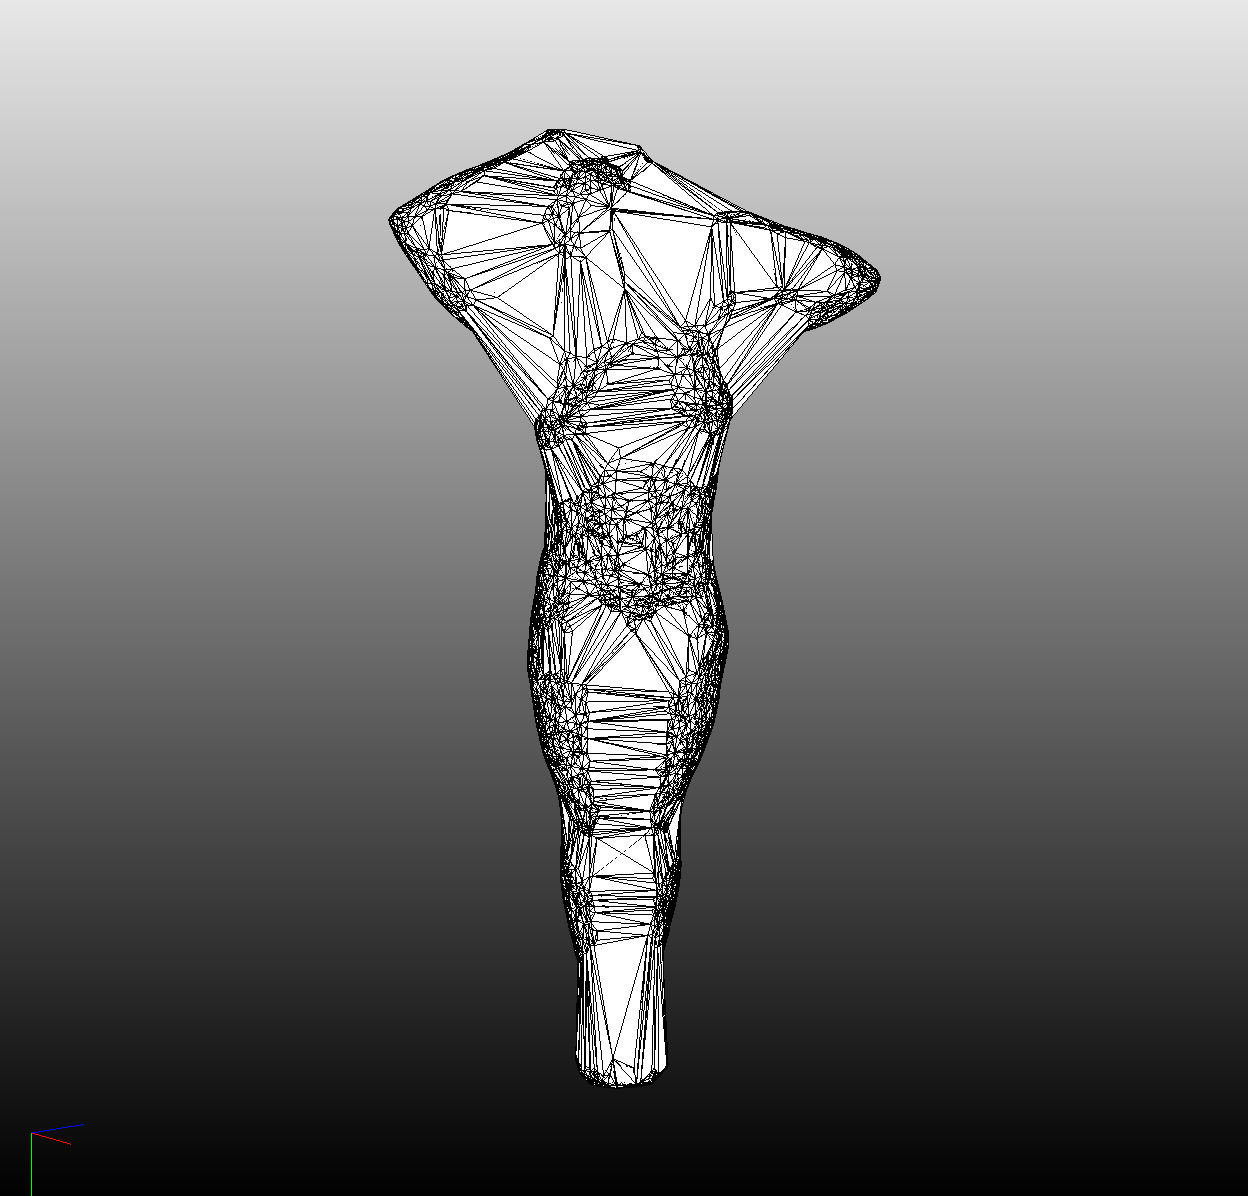
\includegraphics[width=0.32\textwidth]{img/woman2.png}
     \label{fig:woman2}
  }\hspace{-3mm}
  \subfigure[]{
    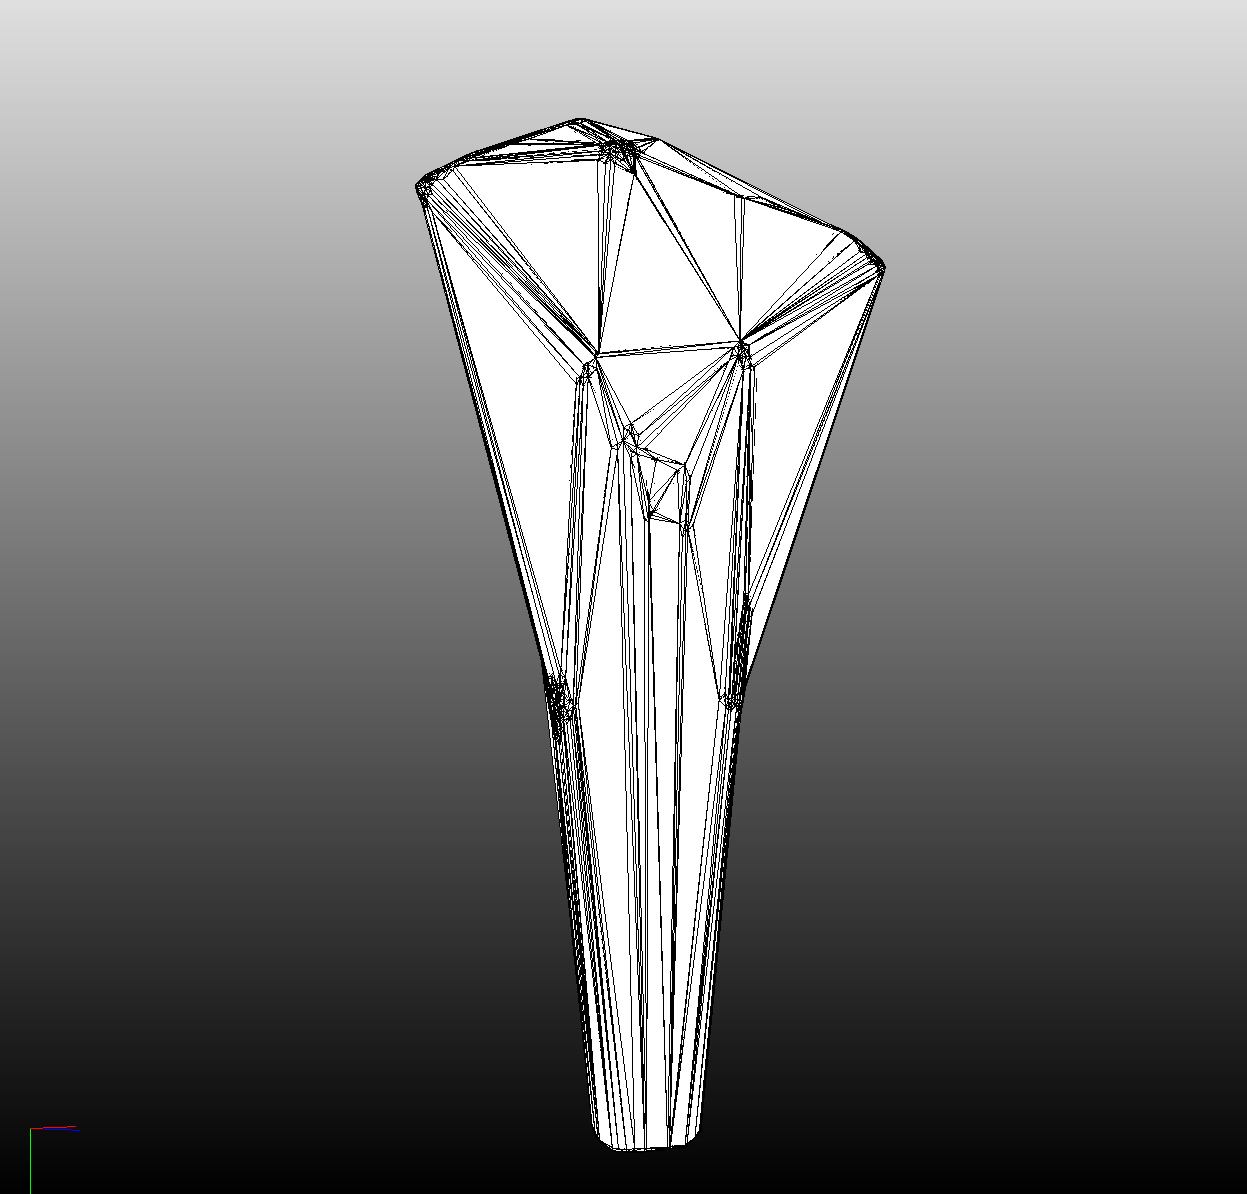
\includegraphics[width=0.32\textwidth]{img/woman3.png}
     \label{fig:woman3}
  }\hspace{-3mm}
  \caption{An woman example \label{fig:woman}}
\end{figure*}
\begin{figure*}[hbt]
 \centering
  \subfigure[]{
    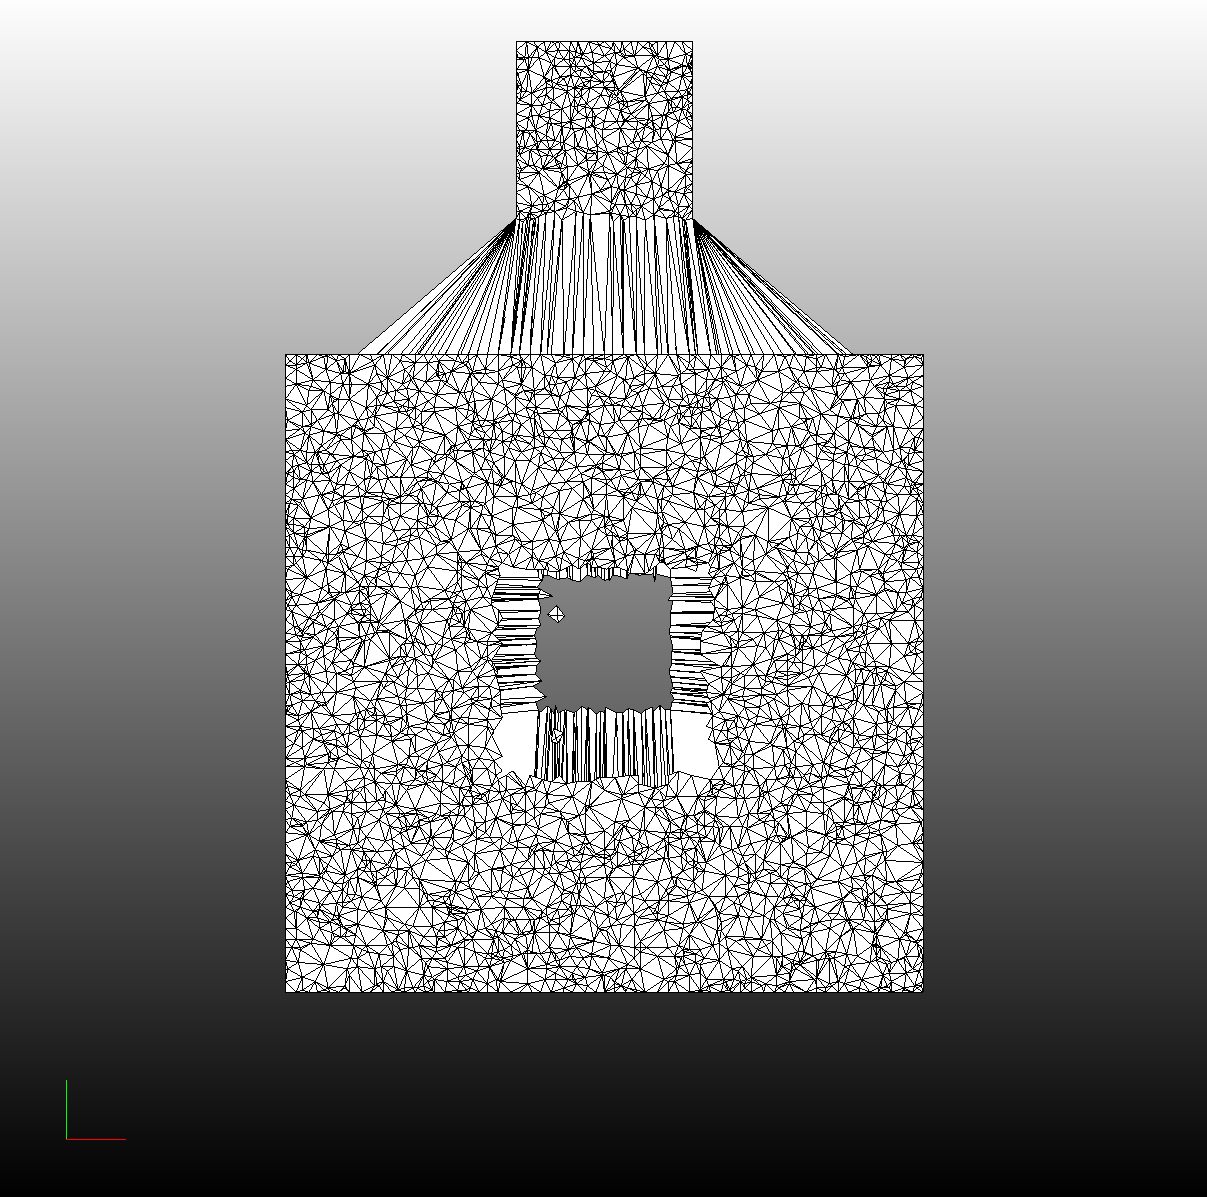
\includegraphics[width=0.32\textwidth]{img/T1.png}
    \label{fig:t1}
  }\hspace{-3mm}
  \subfigure[]{
     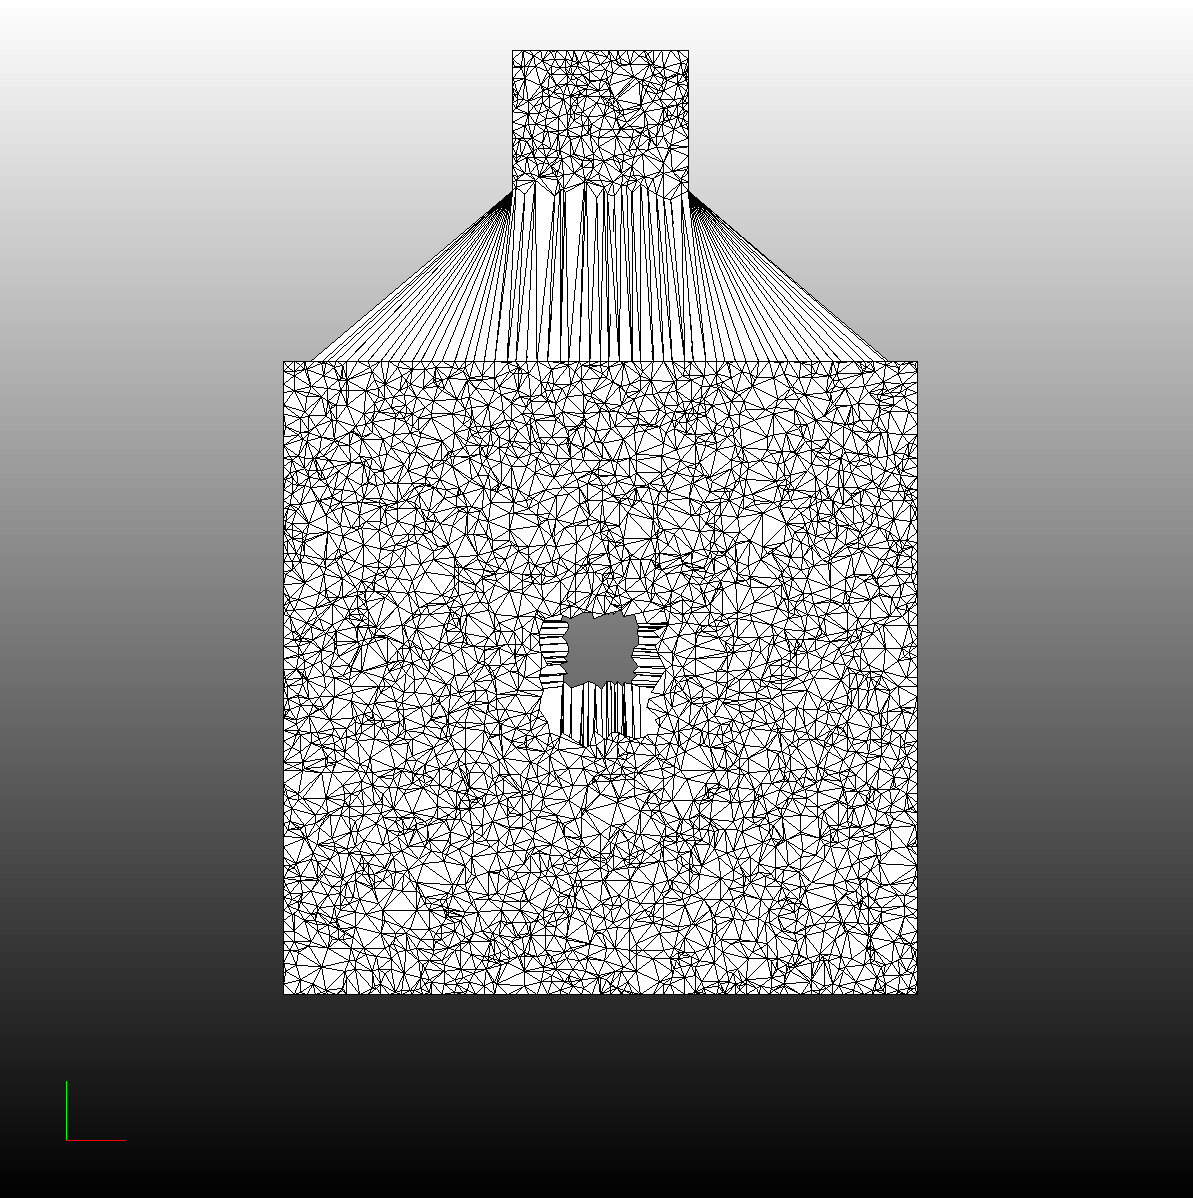
\includegraphics[width=0.32\textwidth]{img/T2.png}
     \label{fig:t2}
  }\hspace{-3mm}
  \subfigure[]{
    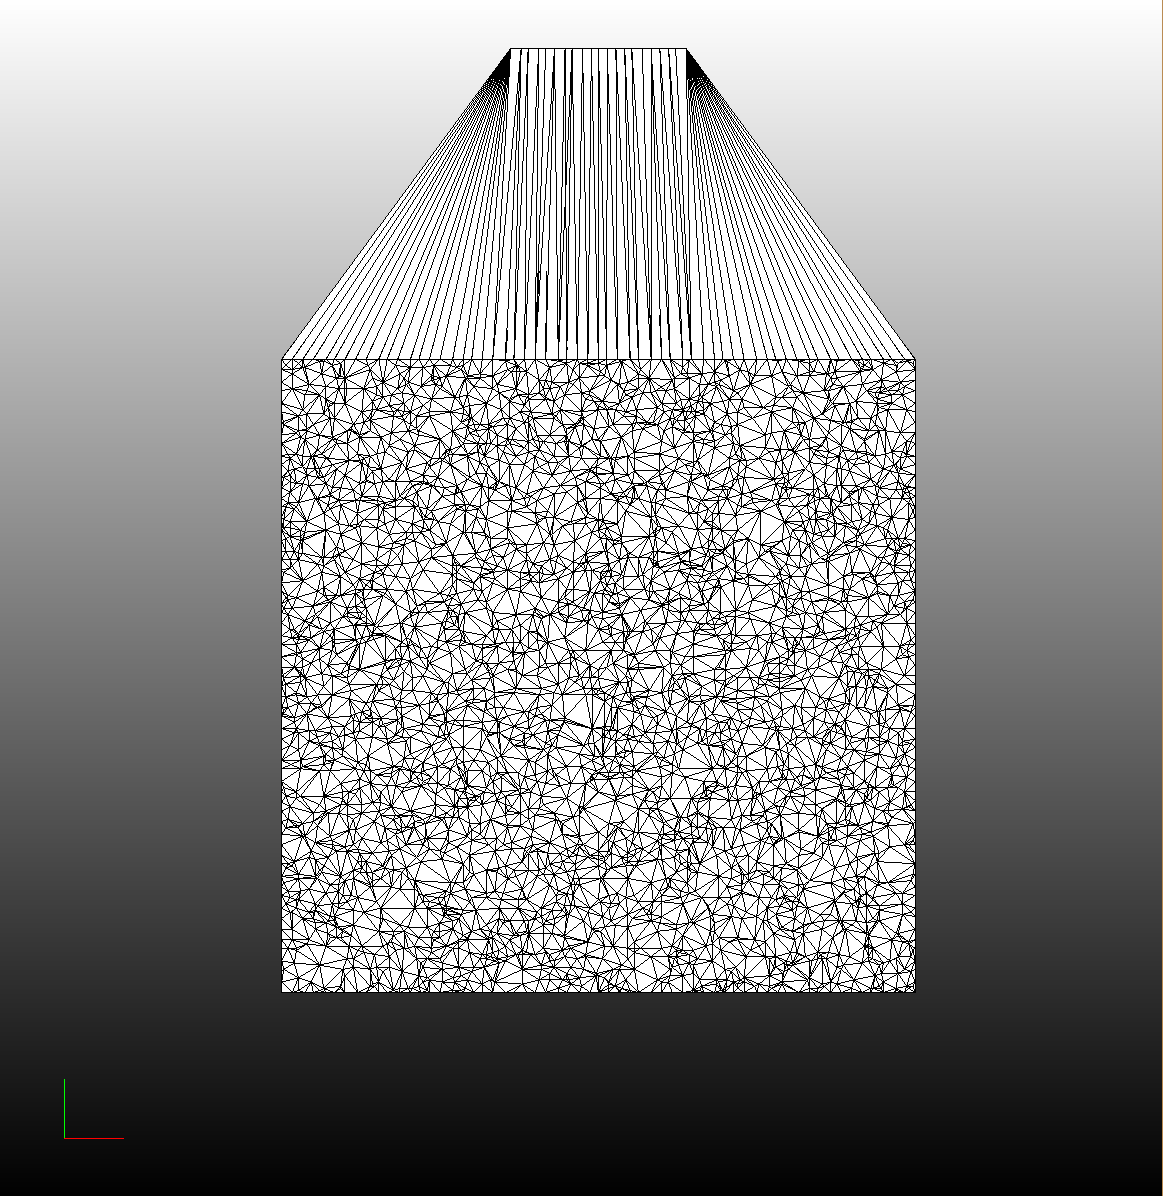
\includegraphics[width=0.32\textwidth]{img/T3.png}
     \label{fig:t3}
  }\hspace{-3mm}
  \caption{A 'T' example \label{fig:T}}
\end{figure*}
\begin{figure*}[hbt]
 \centering
  \subfigure[]{
    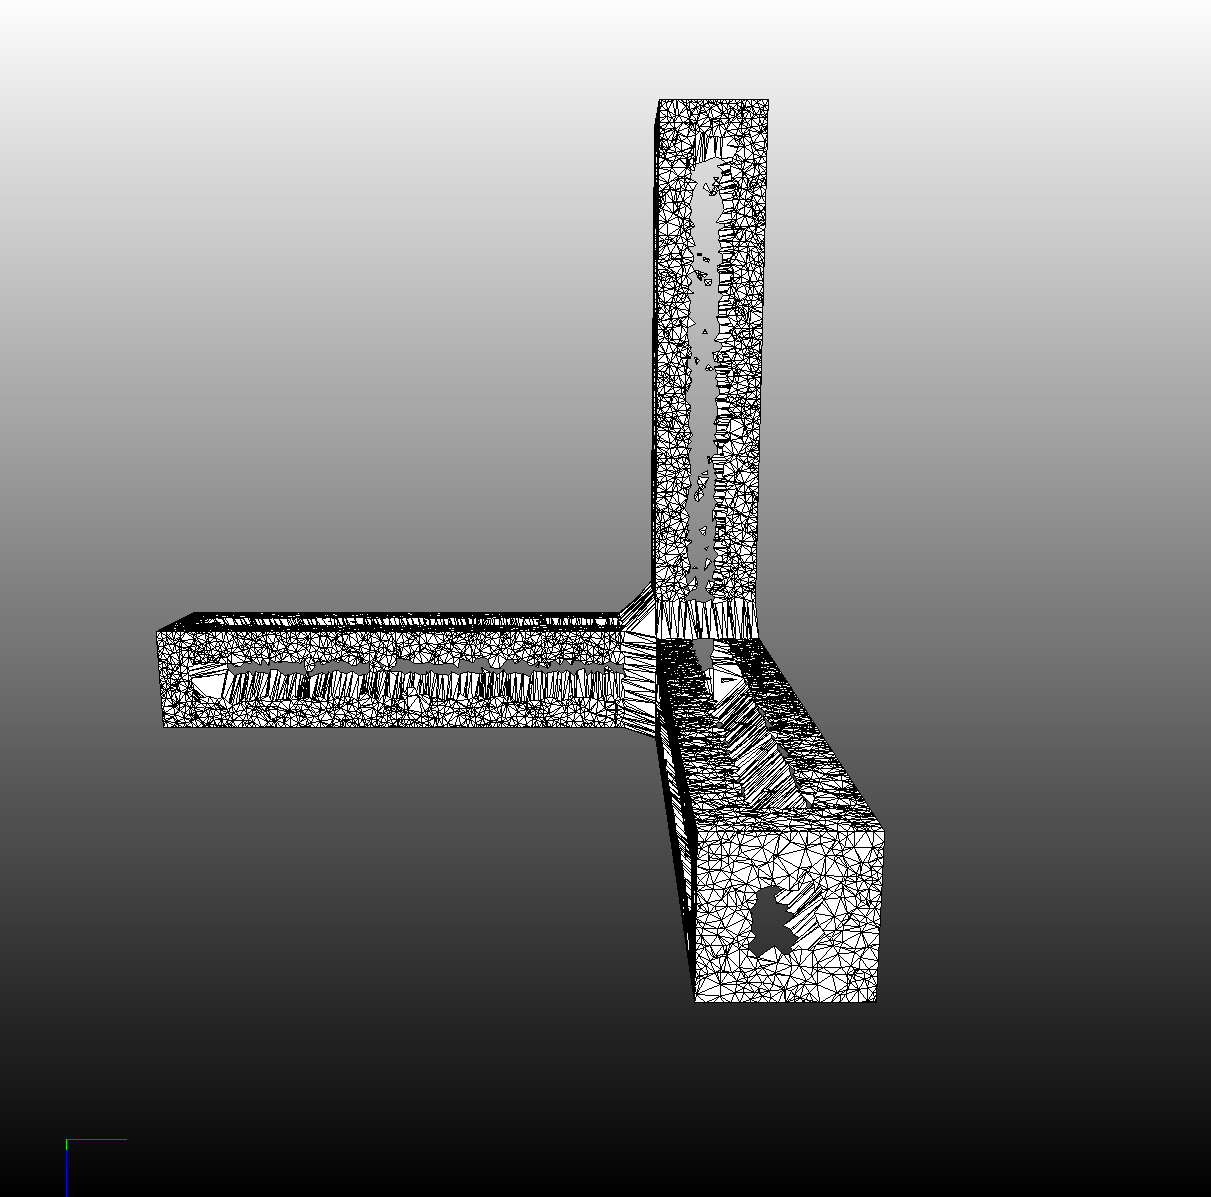
\includegraphics[width=0.32\textwidth]{img/Y1.png}
    \label{fig:y1}
  }\hspace{-3mm}
  \subfigure[]{
     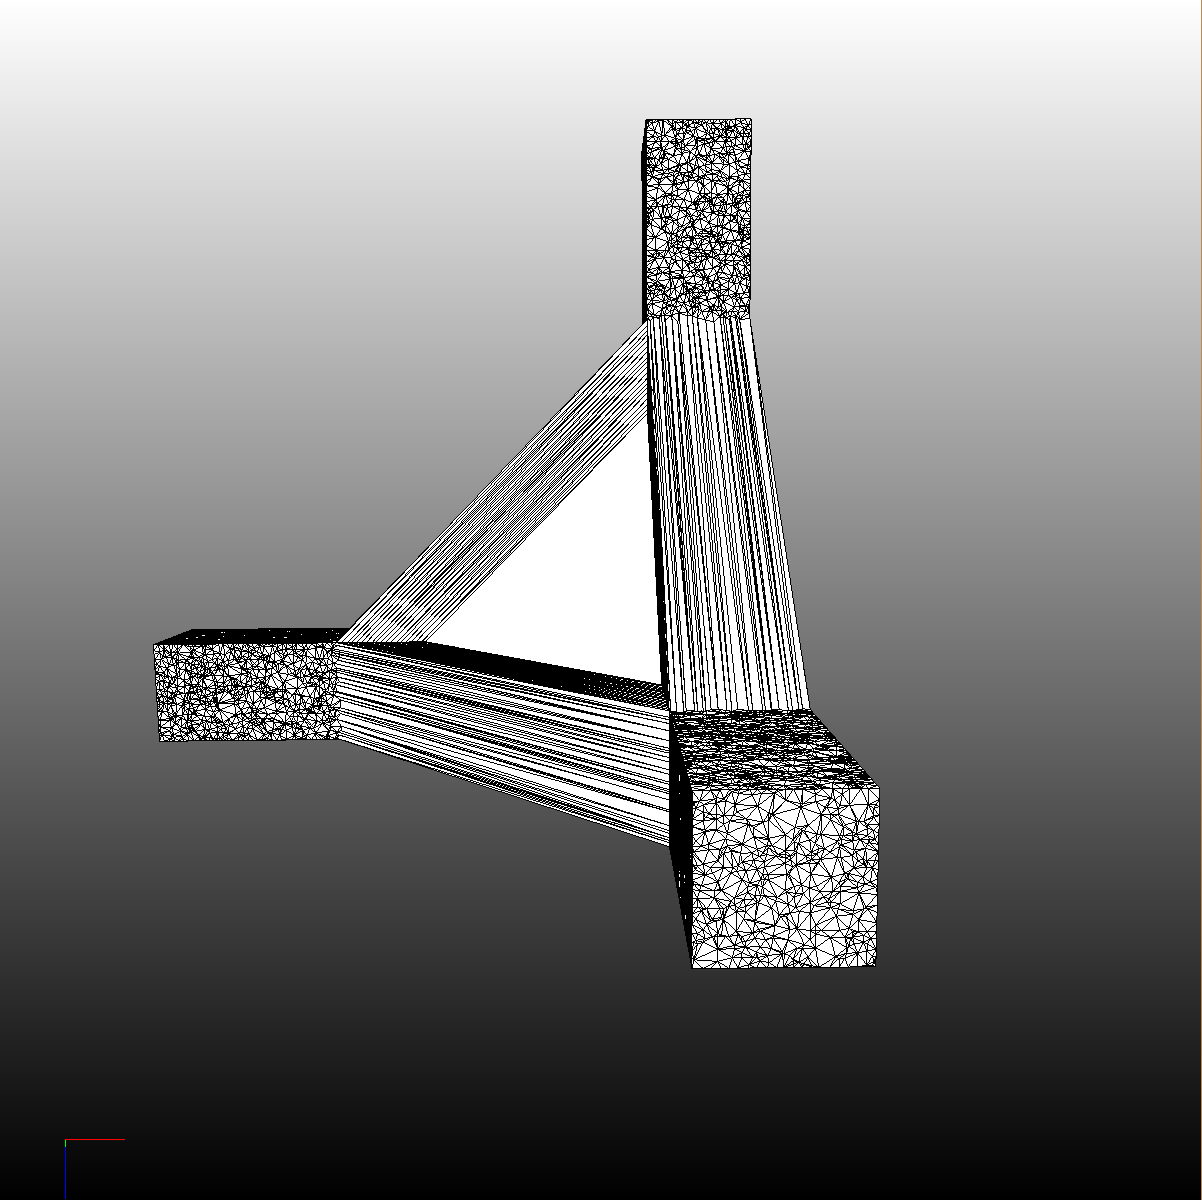
\includegraphics[width=0.32\textwidth]{img/Y2.png}
     \label{fig:y2}
  }\hspace{-3mm}
  \subfigure[]{
    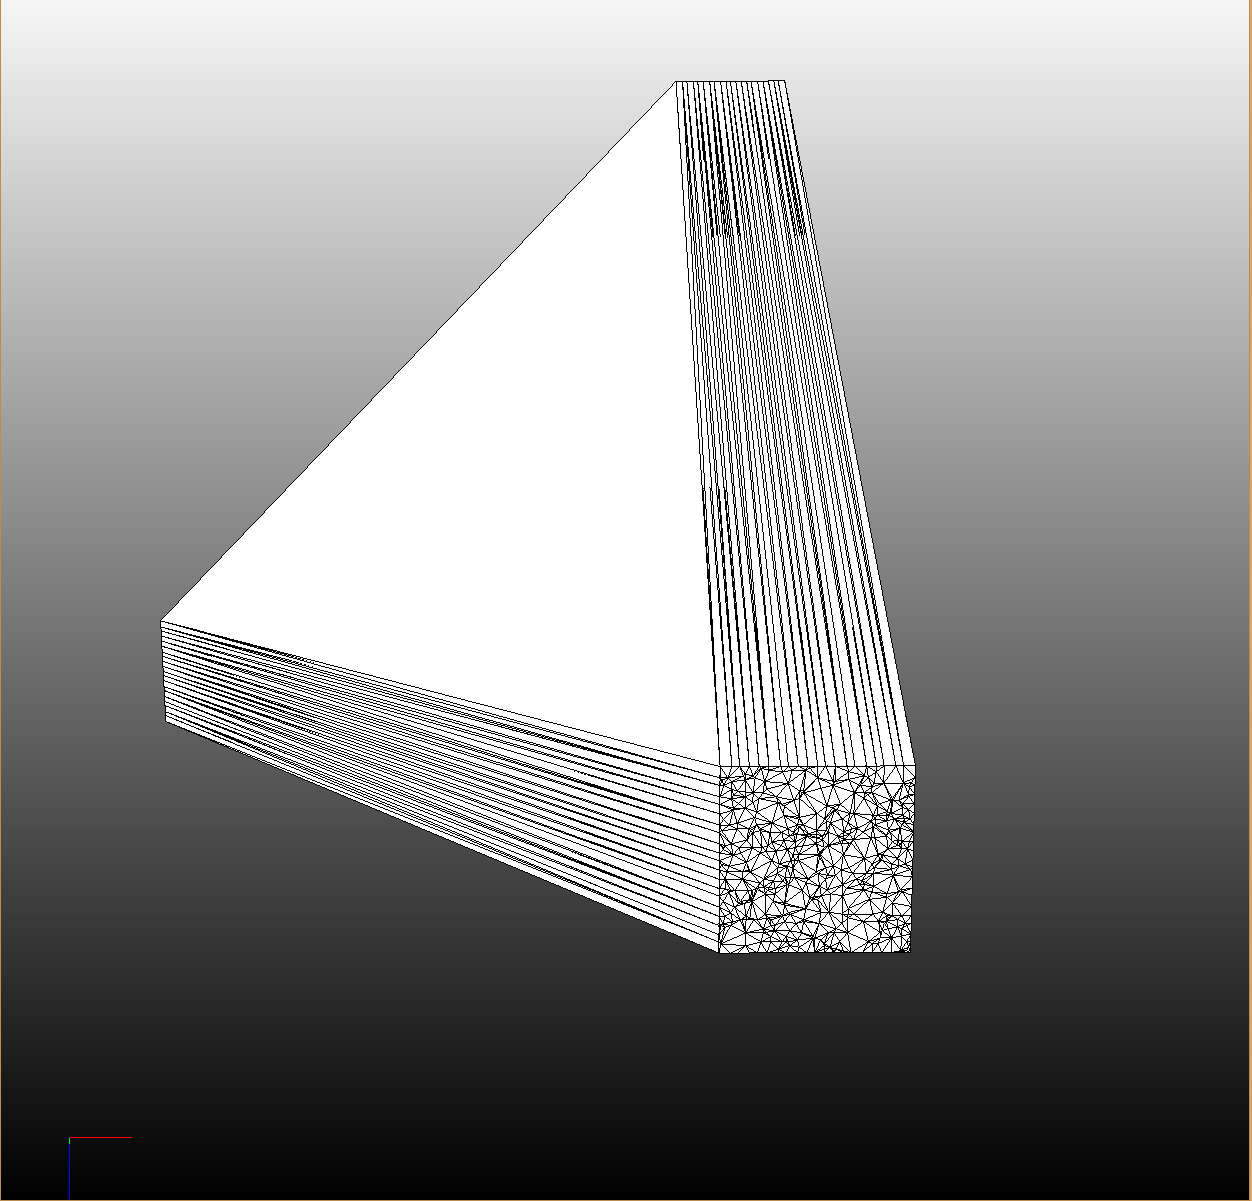
\includegraphics[width=0.32\textwidth]{img/Y3.png}
     \label{fig:y3}
  }\hspace{-3mm}
  \caption{An 'Y' example \label{fig:Y}}
\end{figure*}
\begin{figure*}[hbt]
 \centering
  \subfigure[]{
    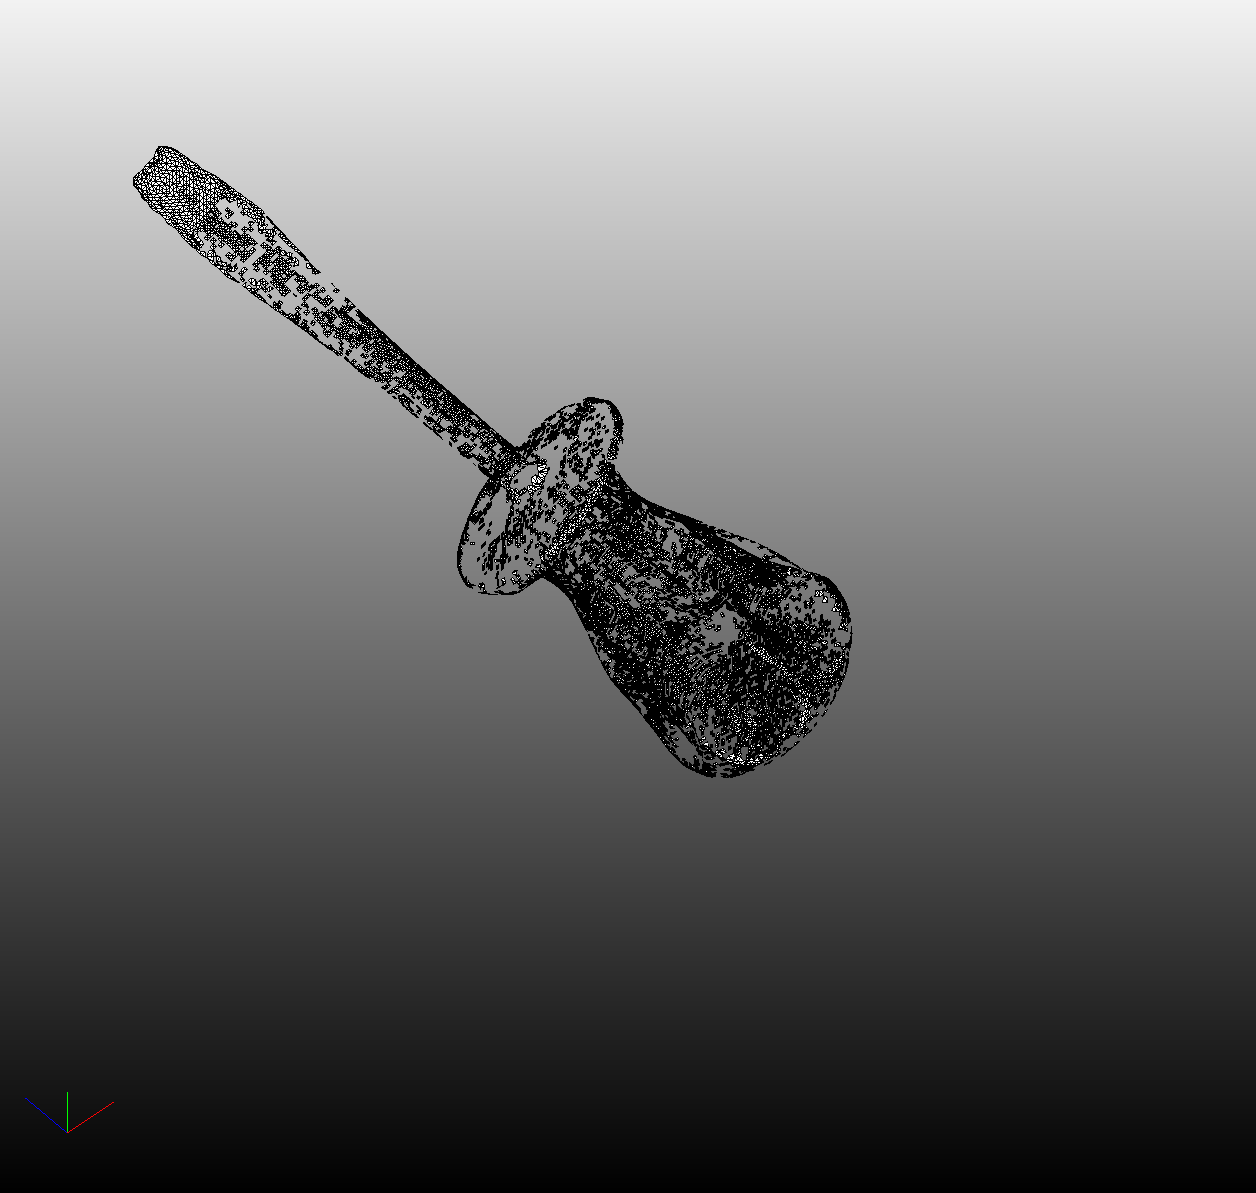
\includegraphics[width=0.32\textwidth]{img/sd1.png}
    \label{fig:sd13}
  }\hspace{-3mm}
  \subfigure[]{
     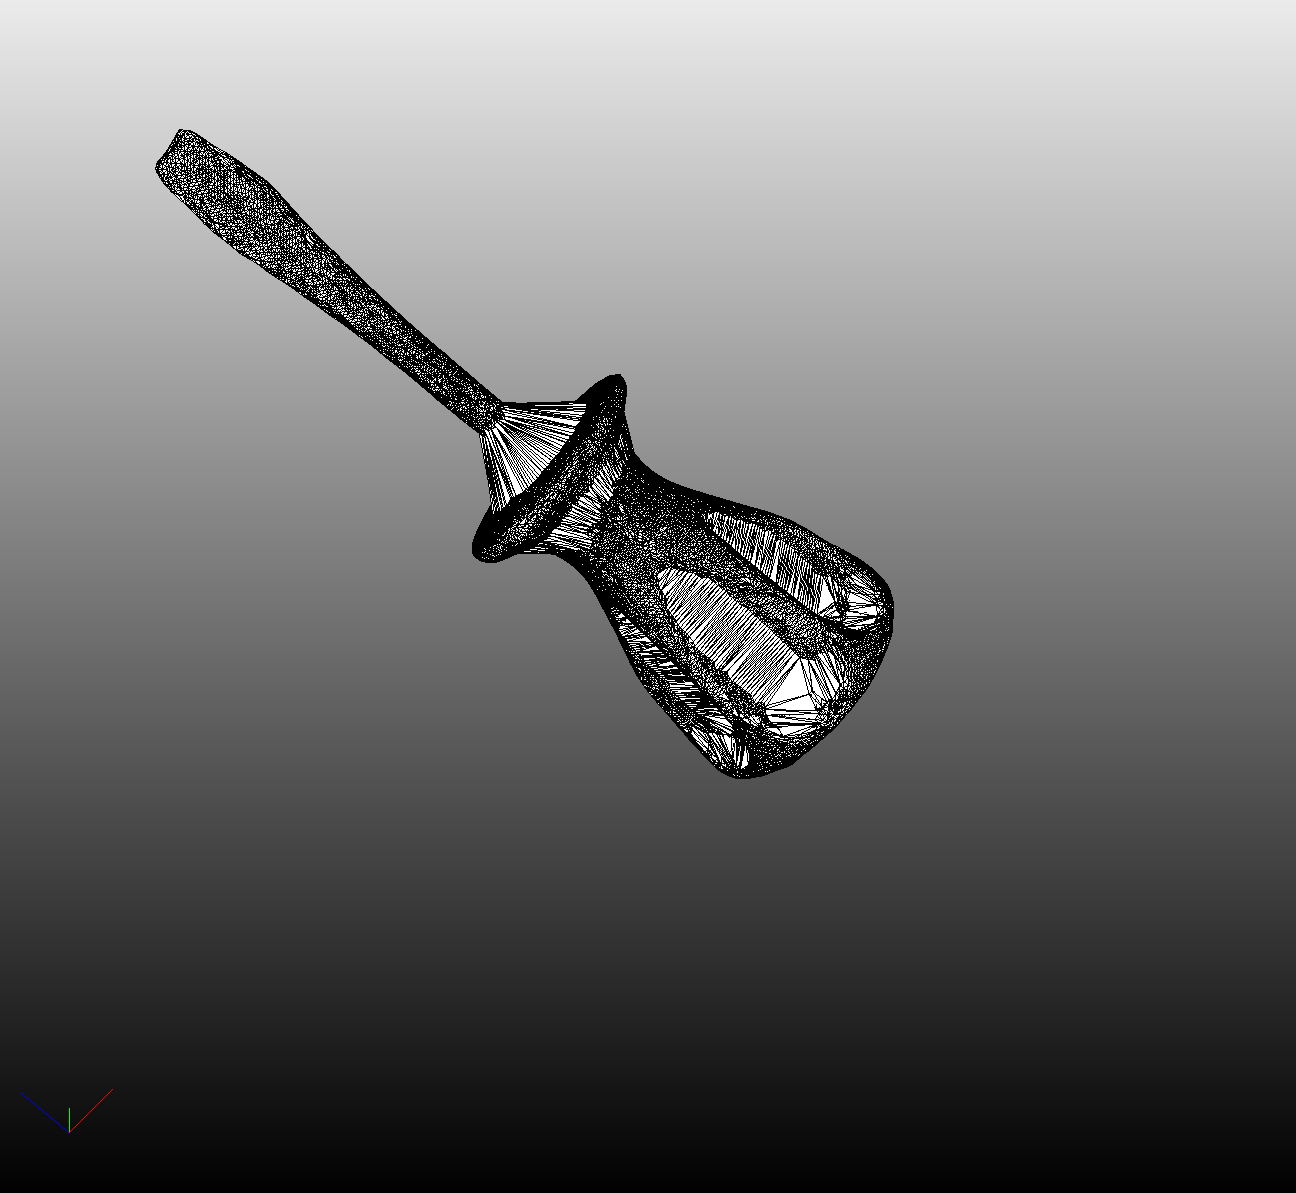
\includegraphics[width=0.32\textwidth]{img/sd2.png}
     \label{fig:sd2}
  }\hspace{-3mm}
  \subfigure[]{
    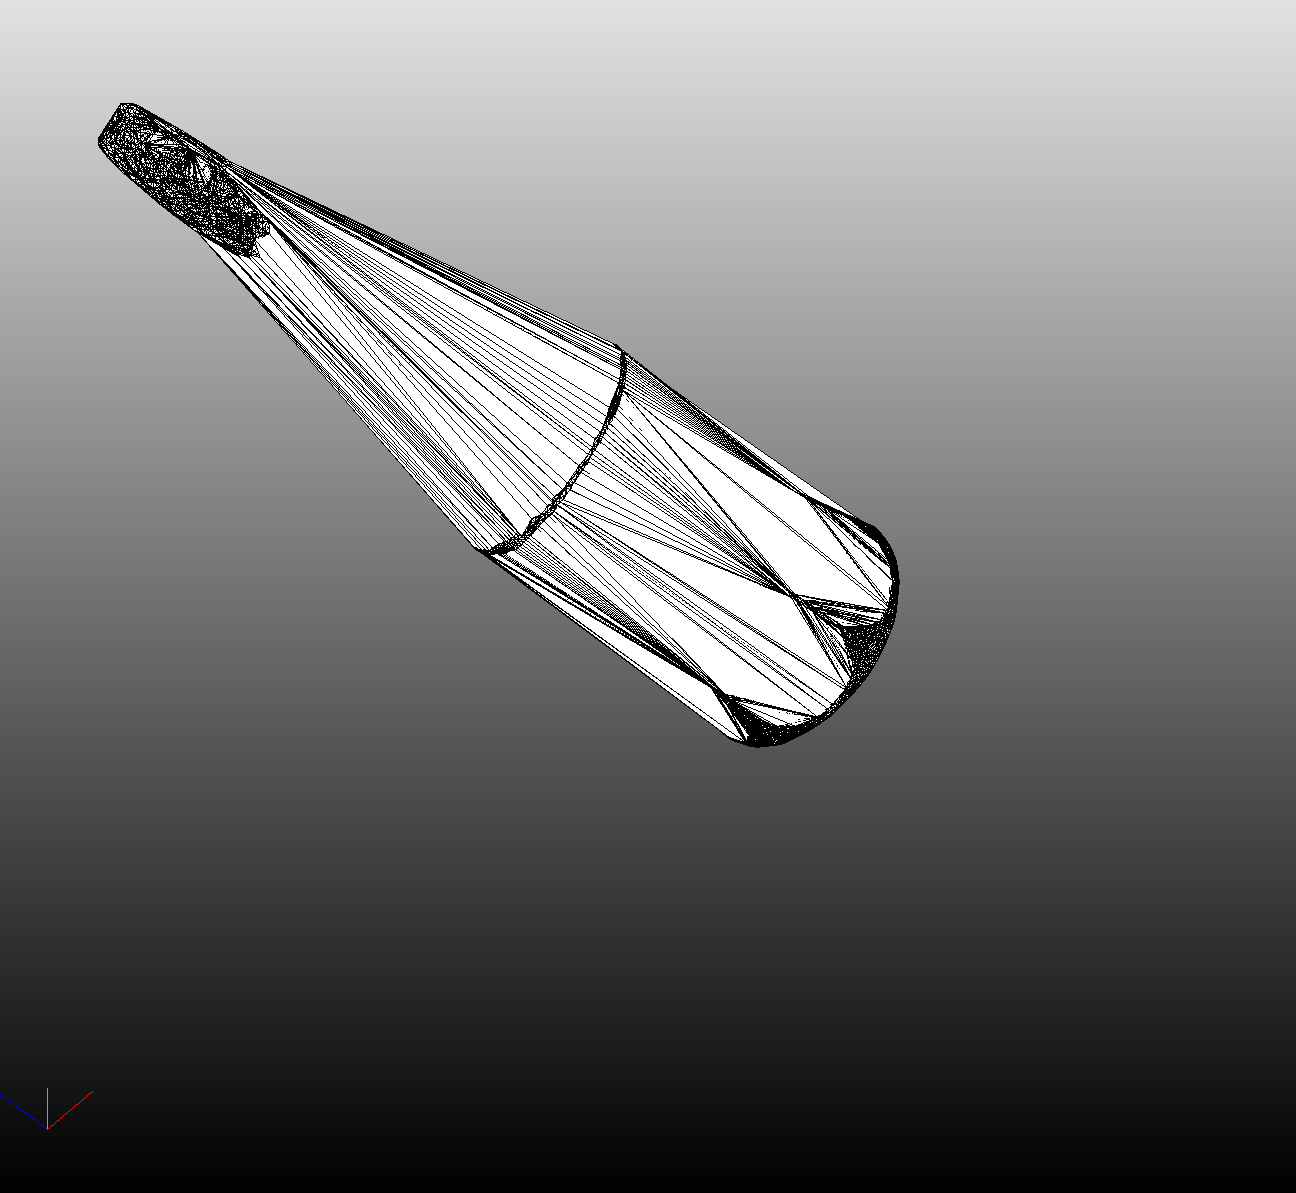
\includegraphics[width=0.32\textwidth]{img/sd3.png}
     \label{fig:sd3}
  }\hspace{-3mm}
  \caption{A screwdriver example \label{fig:sd}}
\end{figure*}
\begin{figure*}[hbt]
 \centering
  \subfigure[]{
    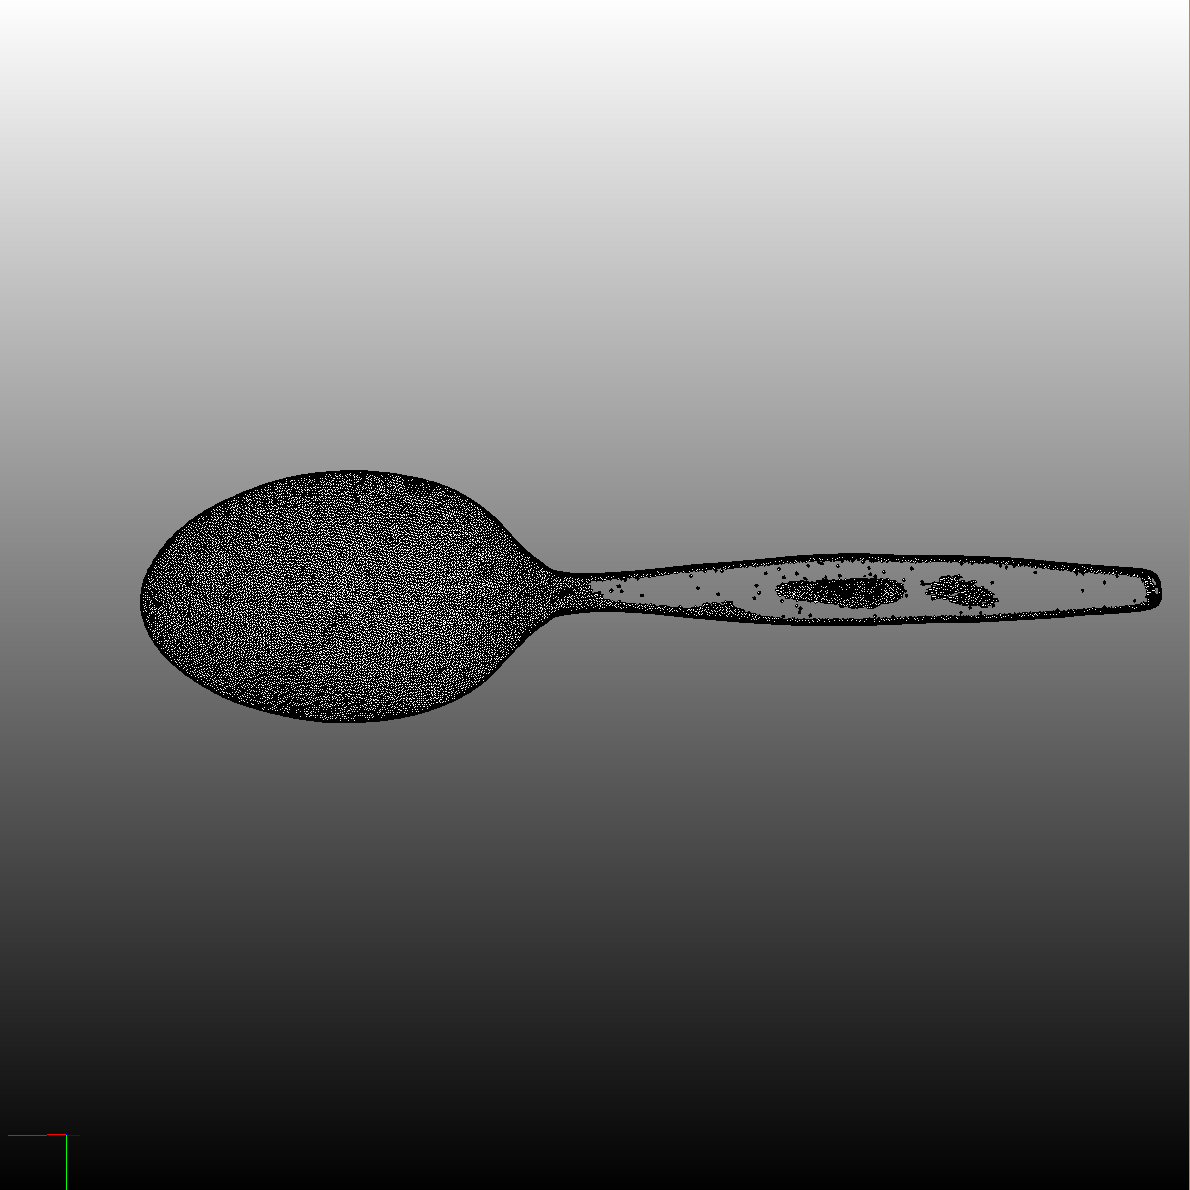
\includegraphics[width=0.32\textwidth]{img/spoon1.png}
    \label{fig:spoon1}
  }\hspace{-3mm}
  \subfigure[]{
     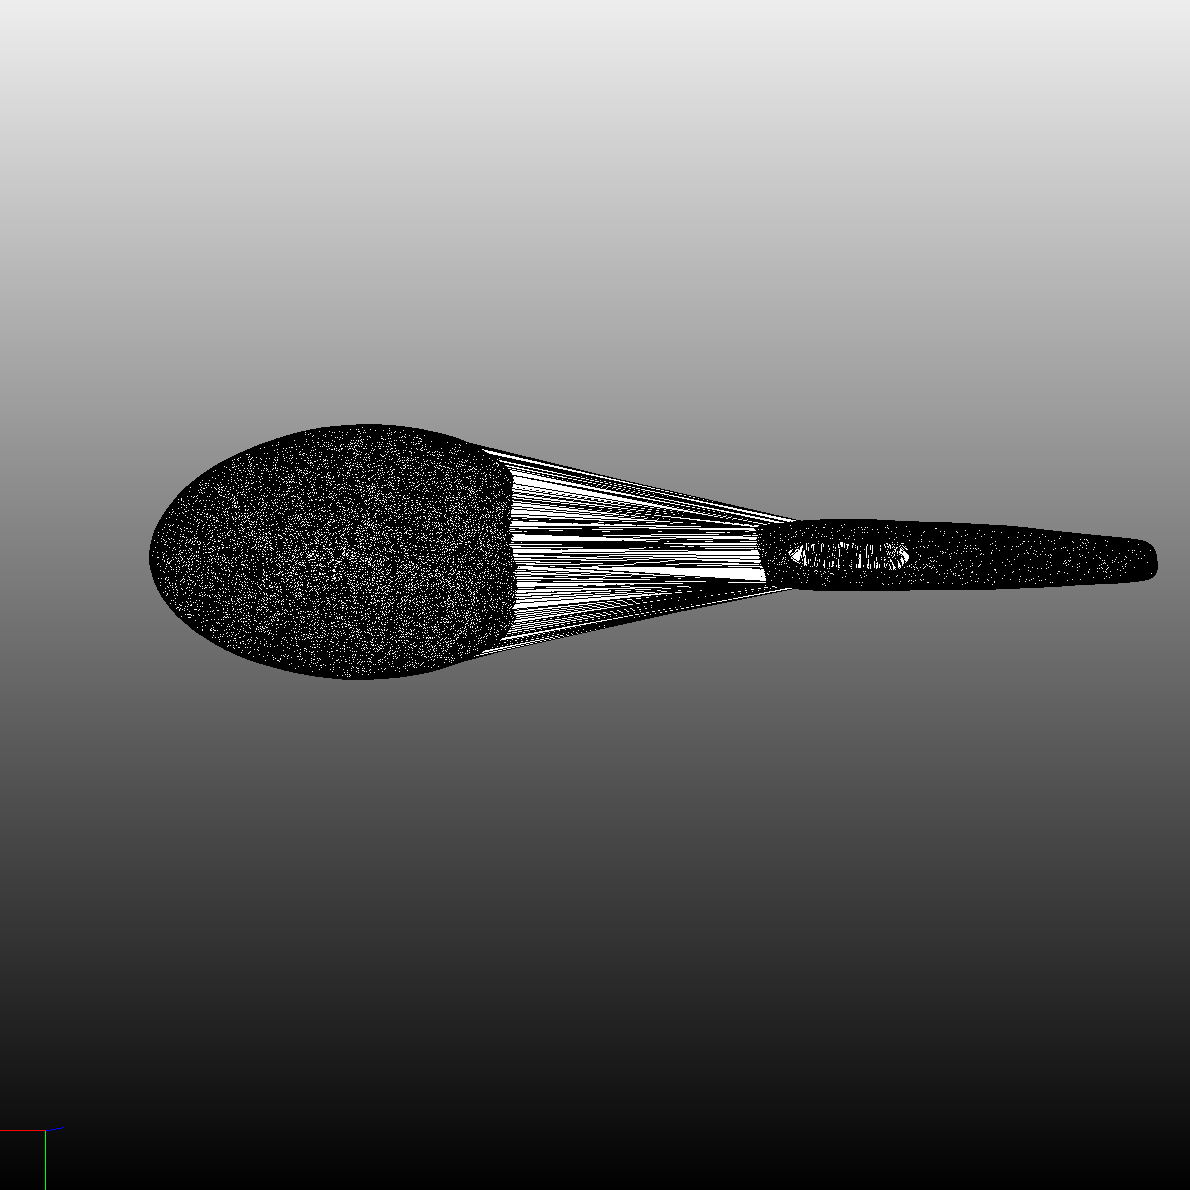
\includegraphics[width=0.32\textwidth]{img/spoon2.png}
     \label{fig:spoon2}
  }\hspace{-3mm}
  \subfigure[]{
    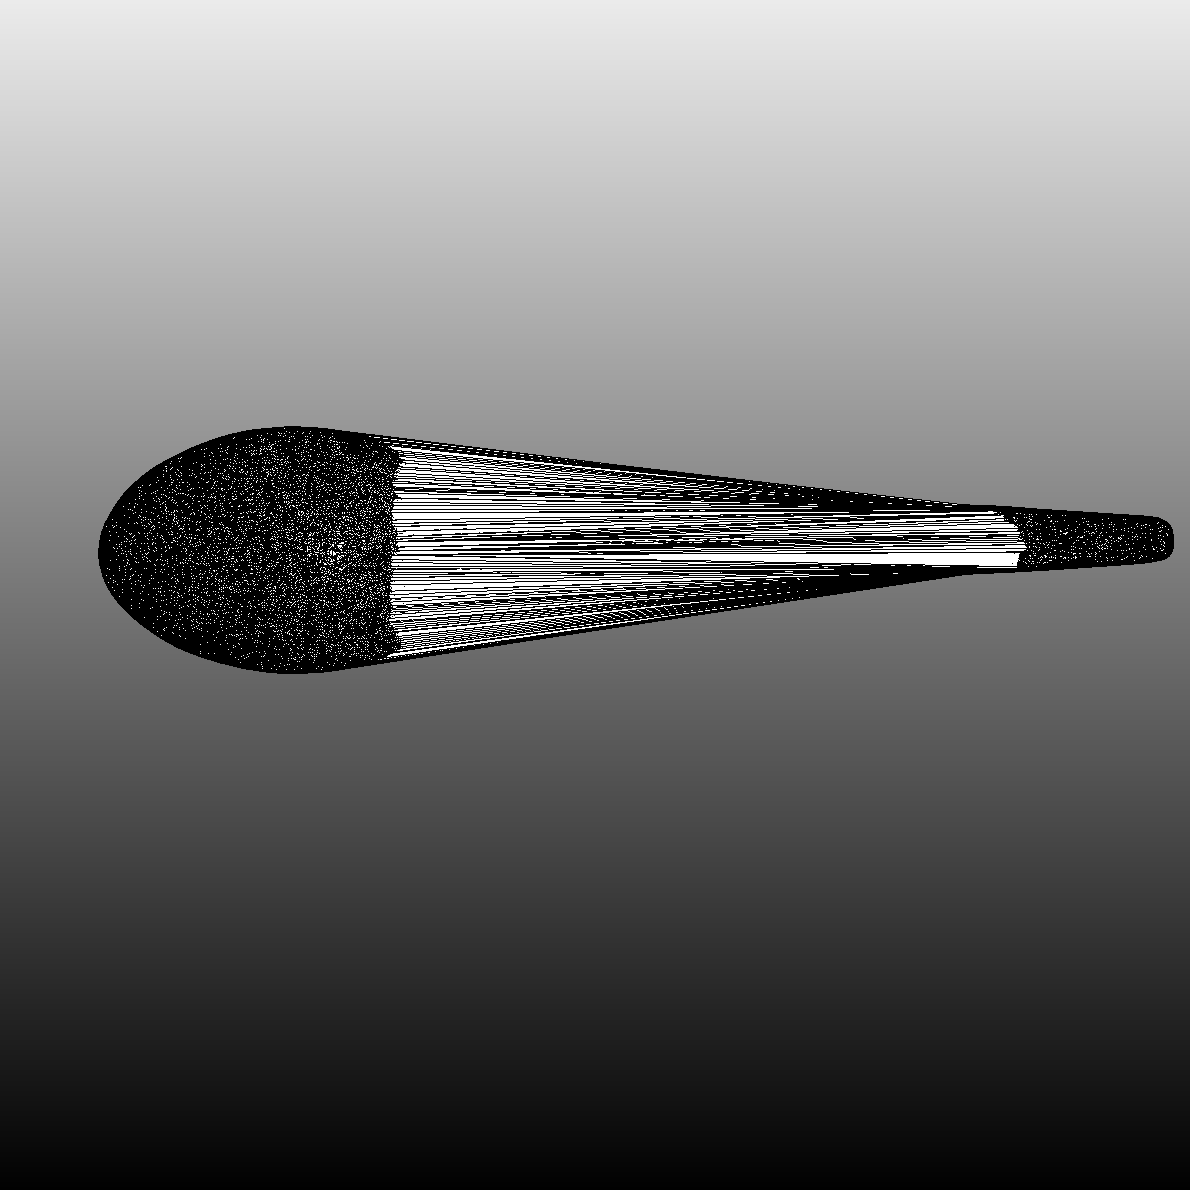
\includegraphics[width=0.32\textwidth]{img/spoon3.png}
     \label{fig:spoon3}
  }\hspace{-3mm}
  \caption{A spoon example \label{fig:spoon}}
\end{figure*}
\begin{figure*}[hbt]
 \centering
  \subfigure[]{
    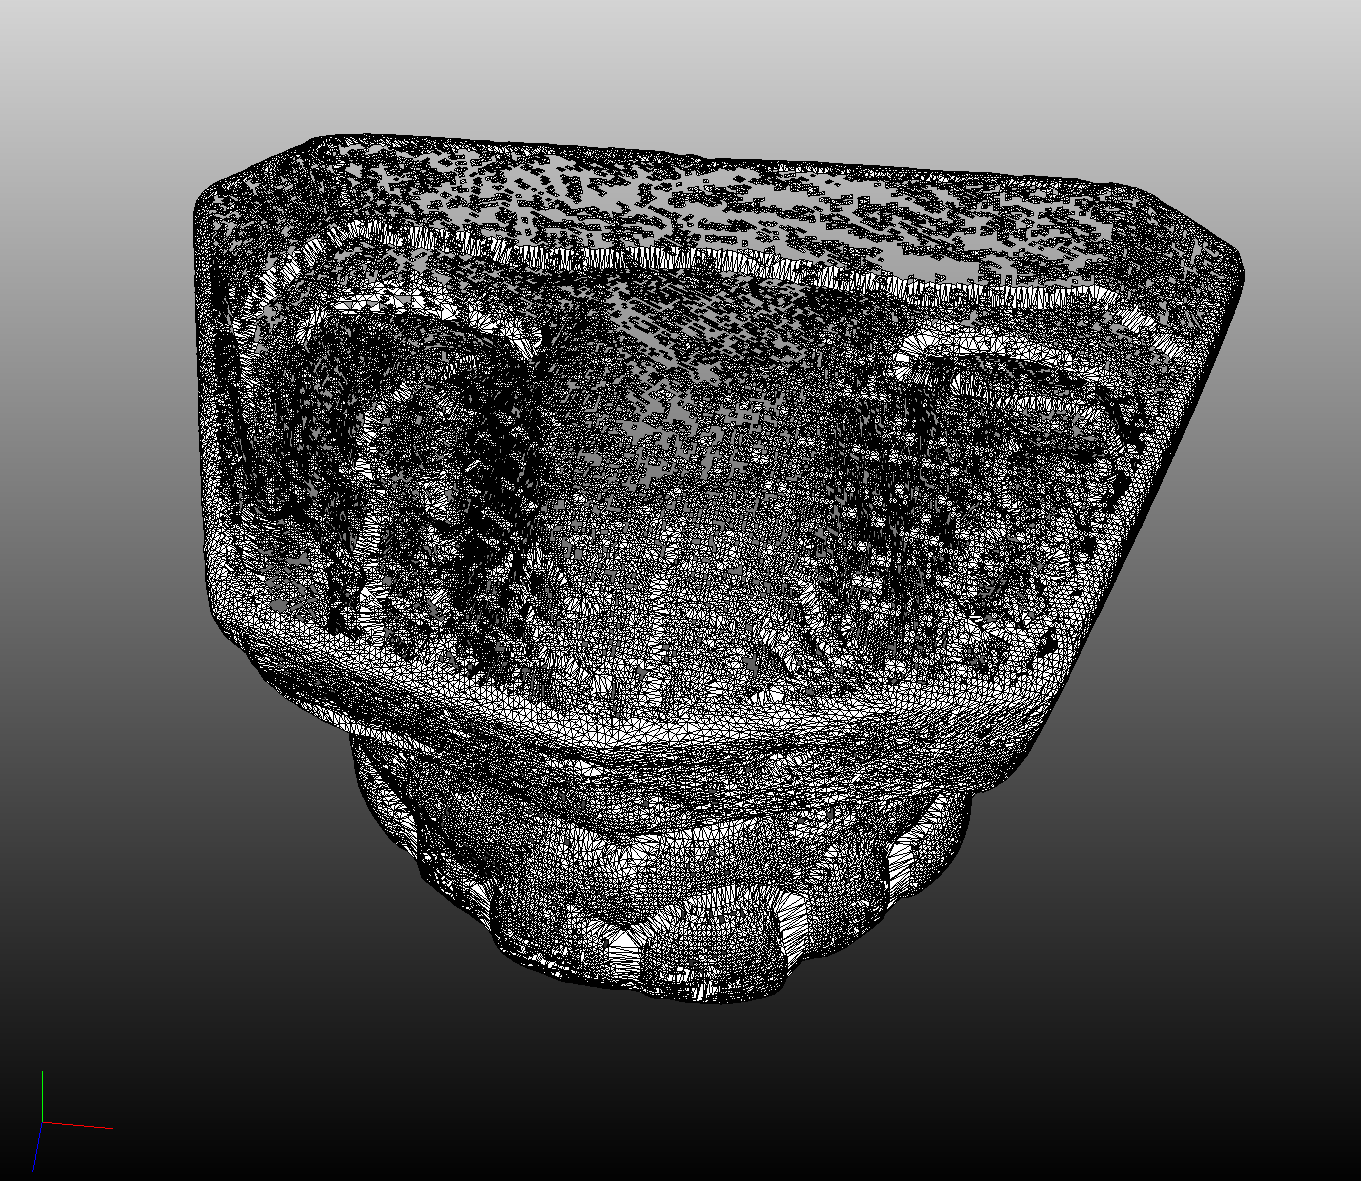
\includegraphics[width=0.32\textwidth]{img/teeth1.png}
    \label{fig:teeth1}
  }\hspace{-3mm}
  \subfigure[]{
     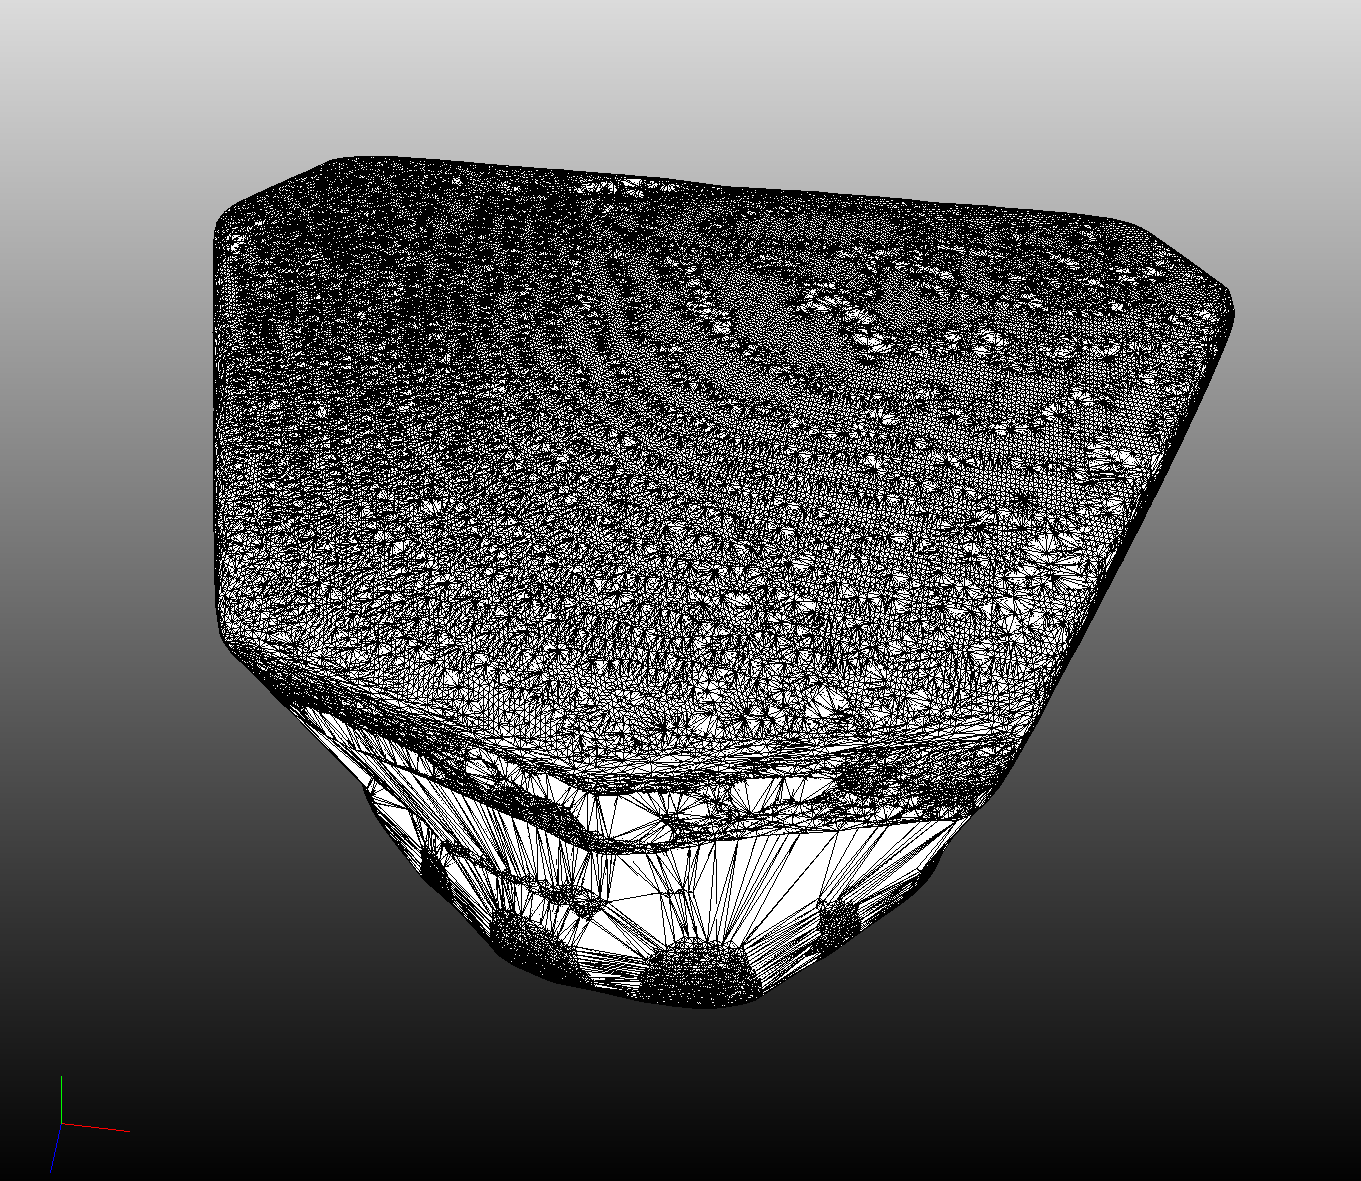
\includegraphics[width=0.32\textwidth]{img/teeth2.png}
     \label{fig:teeth2}
  }\hspace{-3mm}
  \subfigure[]{
    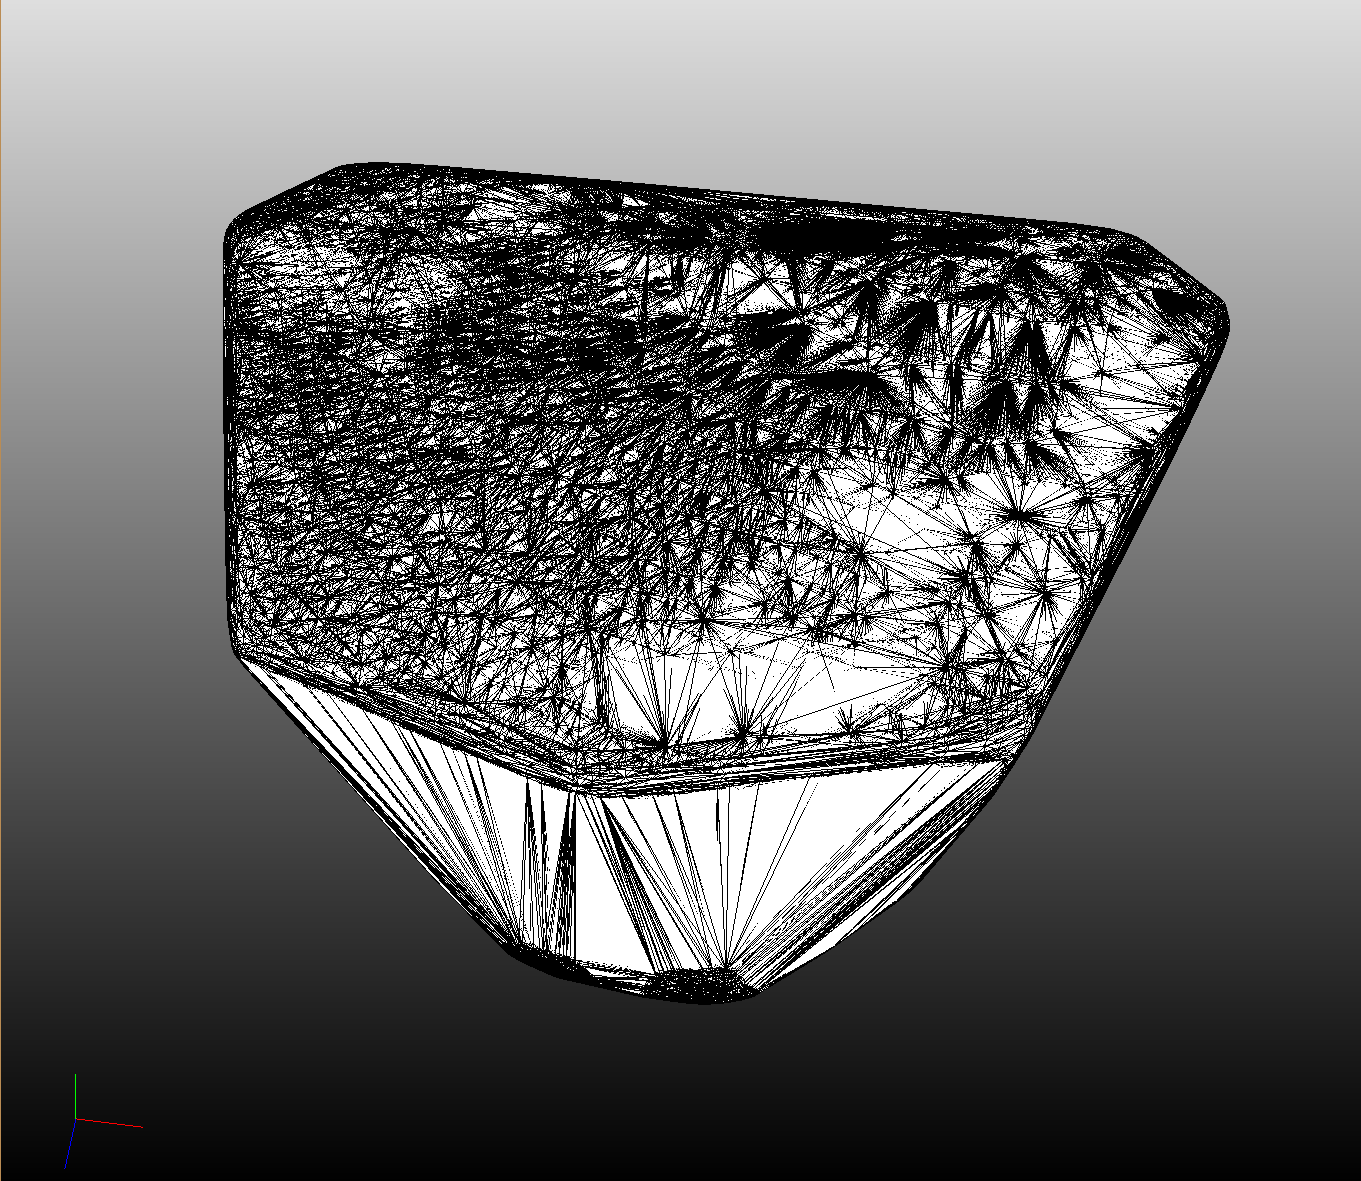
\includegraphics[width=0.32\textwidth]{img/teeth3.png}
     \label{fig:teeth3}
  }\hspace{-3mm}
  \caption{A teeth example \label{fig:teeth}}
\end{figure*}
\end{document}




